\documentclass[a4paper]{article}

% LANGAGE
\input{../latex-std/lang-de.tex}
\input{../latex-std/lang-de-extensions.tex}


% DOCUMENT PRE POST META
\input{../latex-std/doc-pre-post.tex}

\input{../latex-std/doc-biber.tex}
\addbibresource{bibliography.bib}
\addbibresource{KNP11.bib}
\addbibresource{esrel.bib}
\addbibresource{symmetry.bib}
\addbibresource{bisim.bib}
\addbibresource{Par02.bib}
\addbibresource{live.bib}
\addbibresource{chaitin.bib}

% TEXT STRUCTURE ENVIRONMENTS
\input{../latex-std/articul-comments.tex}
\input{../latex-std/articul-structure.tex}


% MATH SYMBOLS
\input{../latex-std/symb-math.tex}

\newcommand{\mc}{Markow-Kette}
\newcommand{\mcpl}{Markow-Ketten}
\title{Syntaxbasierte Reduktion von PRISM Modellen}
\author{Maximilian Starke}
\affil{Fakultät für Informatik, Technische Universität Dresden}
\date{\today}

\usepackage{mathtools}
\usepackage{ragged2e}

\usepackage{framed}
\usepackage{amsmath, amssymb}
\usepackage{tabularx}

\DeclareMathOperator*{\argmin}{\arg\min}

\usepackage{pgfplots}
\pgfplotsset{width=10cm,compat=1.10}
\usepgfplotslibrary{fillbetween}
\newcolumntype{P}[1]{>{\centering\arraybackslash}p{#1}}

\usepackage{listings}
\lstset
{ %Formatting for code in appendix
	basicstyle=\footnotesize,
	numbers=left,
	frame=single
	stepnumber=1,
	showstringspaces=false,
	tabsize=1,
	breaklines=true,
	breakatwhitespace=false,
}
\newcolumntype{M}[1]{>{\centering\arraybackslash}m{#1}}
\newcolumntype{L}[1]{>{\flushleft\arraybackslash}m{#1}}


\usepackage{tikz}

\usetikzlibrary{%
	arrows,
	shapes,
	shapes.misc,% wg. rounded rectangle
	shapes.arrows,%
	chains,%
	matrix,%
	positioning,% wg. " of "
	backgrounds,
	fit,
	petri,
	scopes,%
	decorations.pathmorphing,% /pgf/decoration/random steps | erste Graphik
	shadows,%
	calc
}
%#1
\tikzstyle{vertex}=[circle, minimum size=20pt, line width = 1pt, draw = black]
\tikzstyle{target} = [vertex, double, double distance = 1pt]
\tikzstyle{edge} = [draw,shorten > = 1pt, shorten < = 1pt, line width=1pt,->]
\tikzstyle{medge} = [draw, line width = 8pt, yellow!50]
\tikzstyle{weight} = [font=\small]
\tikzstyle{selected edge} = [draw,line width=5pt,-,red!50]
\tikzstyle{ignored edge} = [draw,line width=5pt,-,black!20]

\usepackage{relsize}

\usepackage{xcolor}
% maybe install minted some day and make syntax highlighting###

\usepackage[utf8]{inputenc}
\usepackage{amsmath, amssymb}

\usepackage[thmmarks,amsmath,hyperref,noconfig]{ntheorem} 
% erlaubt es, Sätze, Definitionen etc. einfach durchzunummerieren.
\newtheorem{satz}{Satz}[section] % Nummerierung nach Abschnitten
\newtheorem{proposition}[satz]{Proposition}
\newtheorem{korollar}[satz]{Korollar}
\newtheorem{lemma}[satz]{Lemma}
\newtheorem{vermutung}[satz]{Vermutung}

\theorembodyfont{\upshape}
\newtheorem{beispiel}[satz]{Beispiel}
\newtheorem{bemerkung}[satz]{Bemerkung}
\newtheorem{definition}[satz]{Definition} %[section]
\newtheorem{algorithmus}[satz]{Algorithmus}

\theoremstyle{nonumberplain}
\theoremheaderfont{\itshape}
\theorembodyfont{\normalfont}
\theoremseparator{.}
\theoremsymbol{\ensuremath{_\Box}}
\newtheorem{beweis}{Beweis}
\newtheorem{beweiss}{Beweisskizze}

\qedsymbol{\ensuremath{_\Box}}

\usepackage{chngcntr}
\counterwithin{figure}{section}

\tikzstyle{block} = [rectangle, draw, fill=blue!40, 
text width=7em, text centered, rounded corners, minimum height=5em, node distance= 4.5cm, line width = 2pt]


\tikzstyle{cblock} = [rectangle, draw, fill=blue!40, 
text width=7em, text centered, rounded corners, minimum height=5em, node distance= 3.0cm, line width = 2pt]


\tikzstyle{line} = [draw, -latex', line width = 1pt]


\tikzstyle{cloud} = [ fill = white, rectangle, draw, rounded corners, node distance=2cm,
minimum height=2.5em]

\pgfdeclarelayer{bg}
%\pgfsetlayers{bg,main}	

\pgfdeclarelayer{foreground}
\pgfdeclarelayer{background}
% tell TikZ how to stack them (back to front)
\pgfsetlayers{bg,background,main,foreground}

\newenvironment{meta}
{\begin{center} \Large \color{red} META: \hspace{2ex} \large \color{blue}}
	{\end{center}}

\begin{document}

% title page:
\maketitle
\vspace{3em}
\tableofcontents
\pagebreak

\section{Kurzfassung}

In vielen die Sicherheit von komplexen Systemen betreffenden Problemstellungen spielen probabilistische Modelle, beispielsweise \mcpl{} mit diskreter Zeitauffassung, eine wichtige Rolle. Im konkreten Beispiel kann die Modellierung einer Flugzeugsteuerung und die Analyse resultierender Modelle auf gewisse Eigenschaften dazu beitragen, Abstürze von Flugzeugen zu verhindern.
Der PRSIM model checker \cite{KNP11} ist ein bekanntes Werkzeug, um jene Modelle auf gewisse Eigenschaften zu untersuchen. Dabei ist die Größe des Modells ein limitierender Faktor, weil mit Modellen zunehmender Größe der Speicher- und Rechenaufwand des PRISM model checkers steigt.
Methoden zur intelligenten Variablenumordnung, welche der PRISM model checker bereits mitbringt, erschöpfen noch lange nicht die Möglichkeiten, Modelle in äquivalente Modelle zu verkleinern \cite{dubslaff2019breaking}.
Es gibt Reduktionsmethoden, welche auf semantischer Ebene agieren, beispielsweise basierend auf Bisimulation \cite{GIVAN2003163} oder Symmetrie \cite{symmetry}.
Methoden zur Reduktion von Modellen basierend auf rein syntaktischer Ebene zu finden, ist bis zu unserem Wissensstand ein noch recht offenes Forschungsfeld.
In bisheriger Forschungsarbeit \cite{dubslaff2019breaking} wurde bereits ein Machbarkeitsbeweis geführt, dass tatsächlich eine Reduktion motiviert durch die Methode der Live Range Analysis aus dem Compilerbau möglich ist und diese eine erhebliche Verkleinerung von Modellen bewirken kann.
Ziel soll es in diesem Forschungsprojekt sein, vorhandene Methoden syntaktischer Reduktion weiter zu untersuchen, mit welchen jene Modelle in solche äquivalente kleinere Modelle umgewandelt werden können, die invariant bzgl. der zu analysierenden bzw. verifizierenden Eigenschaft zueinander und zum ursprünglichen Modell sind.
Im Konkreten werden wir zunächst die bereits vorgestellte Methode der syntaktischen Reduktion \cite{dubslaff2019breaking} erweitern, anschließend die Erweiterung in C++ implementieren und schlussendlich ausgewählte Heuristiken für Graphfärbungen vorstellen und evaluieren hinsichtlich des Einflusses auf die Reduktion von Kontrollflussprogrammen.
Dabei verkleinern wir Modelle durch eine Reduktion der Anzahl der Variablen mittels Zusammenfassung redundanter Variablen. Mittels der Zahl der nodes und states, wie sie der PRISM model checker bei der Verarbeitung des verkleinerten Modells im Log ausgibt, werden wir beurteilen, wie erfolgsbringend eine solche Reduktion ist. Die Zahl der states bezeichnet dabei die Zahl der Zustände des gesamten Modells. Die Zahl der nodes ist nicht immer relevant, jedoch entscheidend für die MTBDD Engine von PRISM \cite{Par02}, welche auf Basis von binären Entscheidungsdiagrammen beruht.
Um die Evaluation von Heuristiken für Graphfärbungen zu ermöglichen, entwickeln wir eine geschickte Implementierung, um all jene minimalen reduzierten Modelle zu finden, welche mit kleinster Anzahl an Variablen auskommen.
Wir werden empirisch an beispielhaften Modellen zeigen, dass die Zahl der nodes und states bei der anschließenden Verarbeitung mit PRISM unter allen erhaltenen minimalen reduzierten Modellen variiert.


\section{Grundlagen}

\subsection{PRISMs Eingabesprache}

Wir betrachten für unsere praktische Implementierung gewählte Beispiele, die als \mcpl{} in der Eingabesprache von PRISM vorliegen. Da unsere Hauptmotivation darin besteht, kleine Modelle zu erreichen, um diese dann mit Software wie PRISM in vernünftiger Zeit verarbeiten zu können, beginnen wir mit einem Beispielmodell in der Eingabesprache von PRISM. Davon ausgehend abstrahieren wir und bestimmen unsere Annahmen. Betrachten wir beispielhaft den Ausschnitt eines Modells in Abbildung \ref{bspeingspr}.

\begin{figure}
\caption{Beispiel Eingabesprache}\label{bspeingspr}
{
	\footnotesize
	\begin{lstlisting}
	dtmc
	
	global cf : [0 .. 5];
	global a : [0 .. 4];
	global b : [0 .. 4];
	global c : [0 .. 4];
	global d : [0 .. 4];
	global e : [0 .. 4];
	
	init
	(cf=0) & (a=0) & (b=1) & (c=2) &
	(d=0 | d=1) & (e=4 | e=2)
	endinit
	
	module some_module
	[goto_1] cf = 0 & a = 0 ->   0.4 : cf' = 1 & a' = 1
	+ 0.6 : cf' = 2 & b' = 3;
	[goto_2] cf = 0 & a = 4 ->   0.2 : cf' = 2 & b' = 4
	+ 0.8 : cf' = 4 & e' = 0;
	...
	...
	[reset1] cf = 3 & e = 0 ->   0.3 : cf' = 0 & (e' = 4 | e' = 2)
	+ 0.7 : cf' = 2 & e' = 0;
	endmodule
	
	formula failure = (e = 0);
	\end{lstlisting}
}
\end{figure}

Wie wir sehen, bestehen unsere Modelle zunächst aus einer Menge von Variablen mit endlichem Zustandsraum sowie einer nichtleeren endlichen Menge von Startzuständen.
Ein Zustand des Modells ist hierbei eine konkrete Zuweisung von Werten zu jeder einzelnen Variablen.
Wir gehen weiterhin von genau einem sogenanntem Modul aus, welches aus einzelnen Transitionen besteht, die der Lesbarkeit wegen Namen wie \textit{goto\_1} oder \textit{reset1} tragen können.
Eine Transition besteht aus einer Eintrittsbedingung, z.B. \texttt{ cf = 0 \& a = 0} im Falle von \textit{goto\_1}, welche erfüllt sein muss ($cf$ und $a$ werden gelesen), damit die Transition auf einen Zustand anwendbar ist sowie einer Wahrscheinlichkeitsverteilung für Folgezustandsbedingungen:
Beispielsweise wird bei Eintreten von Transition \textit{goto\_1} mit Wahrscheinlichkeit $0.4$ der Zustand eingenommen, in welchem sich $cf$ zu $1$ ändert und $a$ zu $1$, mit Wahrscheinlichkeit $0.6$ der Zustand, in welchem sich $cf$ zu $2$ ändert und $b$ zu $3$. In letzterem Fall werden $cf$ und $b$ geschrieben.
Mit der Zeile \texttt{formula failure = (e = 0)} wird eine Eigenschaft beschrieben, welche ein Zustand des Modells jeweils erfüllt oder nicht. Somit wird letztlich eine Teilmenge von Zuständen ausgezeichnet. Mit der Verwendung dieser in PCTL-querys lässt sich ein Modell mit dem PRISM model checker auf eine gewünschte Eigenschaft hin untersuchen.

\paragraph{Annahmen an das Modell}


Wir können zusammenfassend sagen, dass die Semantik eines betrachteten Modells jeweils eine \mc{} ist.
In folgenden Abschnitten werden wir uns nur noch auf die syntaktische Ebene beziehen und die Modelle schlicht als Programme mit Variablen auffassen.
Während für allgemeine Betrachtungen Wahrscheinlichkeiten als ein Wesensmerkmal von \mcpl{} von Relevanz sind, können wir diese für unser Vorhaben der Modellreduktion vernachlässigen.
Die Reduktion, welche wir betrachten wollen, basiert auf dem Zusammenführen von Variablen mit disjunkten live ranges, wie es aus dem Compilerbau bekannt ist.
Um die Invarianz bezüglich der durch PRISM zu untersuchenden Eigenschaft herzustellen, ermöglichen wir es, ausgewählte Variablen von der Zusammenführung auszuschließen. Wir wollen die folgenden Annahmen für unsere Reduktion treffen:

\begin{enumerate}[(a)]
	\item Es gibt eine Variable, die als Kontrollflussvariable dient, wir nennen diese hier $cf$ (engl. für \textit{control flow}).
	\item In jeder Transition ist $cf$ in der Eintrittsbedingung eindeutig festgelegt. In allen Folgezustandsbedingungen steht $cf$ eindeutig fest: Dazu bekommt $cf$ entweder explizit einen eindeutigen Wert zugewiesen oder bleibt unverändert.
	\item Es gibt eine Liste von Variablen, die von der Reduktion auszuschließen sind.
\end{enumerate}

Man kann solche Programme auch als \textit{control flow programs} bezeichnen.
Das Beschränken auf die syntaktische Ebene entspricht einer Überapproximation der Liveness.
Führen wir Modellreduktionen mittels live ranges auf der syntaktischen Ebene durch, so führt dies zu keinen unzulässigen Reduktionen im originalen Modell.
Wir verzichten darauf, dies hier formal zu zeigen, weil die Korrektheit intuitiv anhand nachfolgender Darstellungen klar ist. Für eine formale Betrachtung verweisen wir auf \cite{ThesisDubs}.


Um mit der Reduktion von einem Modell zu beginnen, gehen wir also davon aus, dass gegeben sind:
\begin{itemize}
	\item Variablen mit jeweils endlichem Wertebereich $cf \in D_{cf}, x_1 \in D_{1}, x_2, \in D_2, \dots, x_n \in D_n$.
	\item endlich viele Transitionen $t_1, t_2, \dots , t_m$ als Paare von Eintrittsbedingung und Tupel der Folgezustandsbedingungen:
	\[t_i = (f^{enter}_i, (f^{leave}_{i,1}, f^{leave}_{i,2}, \dots , f^{leave}_{i,k_i}))\]
	\item eine Startzustandsbedingung siehe Zeile 10 des Beispielmodells (Abbildung \ref{bspeingspr}).
\end{itemize}

In der vorangegangenen Forschungsarbeit \cite{dubslaff2019breaking} wurden alle Folgezustandsbedingungen einer Transition zu einer Transition zusammengefasst.
Die erste, jedoch natürlich offensichtliche Optimierung, die wir vornehmen wollen, ist es, jede Transition aus der Eingabesprache von PRISM mit mehr als einer Folgezustandsbedingung anhand ebendieser in eigenständige Transitionen aufzusplitten. Dies können wir ohne Weiteres tun, da für unsere auf rein syntaktischer Basis funktionierende Reduktion den Wahrscheinlichkeiten keine Bedeutung zukommt.
Aus 
\begin{equation*}
t_i = (f^{enter}_i, (f^{leave}_{i,1}, f^{leave}_{i,2}, \dots , f^{leave}_{i,k_i}))
\end{equation*}

werden somit die eigenständigen Transitionen

\begin{align*}
t_i^1 & = (f^{enter}_i, (f^{leave}_{i,1})) \\
t_i^2 & = (f^{enter}_i, (f^{leave}_{i,2})) \\
& \dots \\
t_i^{k_i} &= (f^{enter}_i, (f^{leave}_{i,k_i}))
\end{align*}

Daraus können wir unmittelbar einen Kontrollflussgraphen aufbauen, welcher für sich gesehen nur noch die syntaktische Ebene des Modells repräsentiert.

\newcommand{\mgtup}{$G = (V,E,\cdot_{\mathrm{from}}, \cdot_{\mathrm{to}})$}
\newcommand{\subfrom}{_{\mathrm{from}}}
\newcommand{\subto}{_{\mathrm{to}}}
\begin{definition}[Multigraph]
	Sei $V \neq \emptyset$ eine nichtleere Menge, aufgefasst als Menge von Knoten und $E$ eine Menge, aufgefasst als Menge gerichteter Kanten.
	Seien weiterhin
	\begin{align*}
	\cdot_{\mathrm{from}} &: E \to V : e \mapsto e_{\mathrm{from}}\text{,} \\
	\cdot_{\mathrm{to}} &: E \to V : e \mapsto e_{\mathrm{to}}
	\end{align*}
	zwei Abbildungen, die jeder Kante $e$ ihren Startknoten $e_{\mathrm{from}}$ sowie ihren Endknoten $e_{\mathrm{to}}$ zuordnen.
	Dann nennen wir $G = (V,E,\cdot_{\mathrm{from}}, \cdot_{\mathrm{to}})$ einen (gerichteten) Multigraph.
	
\end{definition}

Wir identifizieren jede resultierende Transition als ein $e^j = (f_j^{enter}, f_j^{leave}) \in E$.
Dann erhalten wir unmittelbar einen Multigraphen $G = (V,E,\cdot_{\mathrm{from}}, \cdot_{\mathrm{to}})$ als Programmgraphen, wie wir ihn als Ausgangspunkt für die Live Range Analysis benötigen, indem wir weiterhin definieren: 

\begin{enumerate}[(a)]
	\item $V\coloneqq D_{cf}$
	\item $\forall e^j \in E : e^j_{\mathrm{from}} \coloneqq v_1\text{, falls } f_j^{enter} \implies cf = v_1$
	\item $\forall e^j \in E : e^j_{\mathrm{to}} \coloneqq v_2\text{, falls } f_j^{leave} \implies cf = v_2$
\end{enumerate}

Es sei bemerkt, dass (b) und (c) eindeutig definiert sind aufgrund unserer Annahmen. Wir operieren insofern auf einem semantischen Aspekt des Modells, als dass wir den Zustandsraum $D_{cf}$ einbeziehen müssen. Ansonsten haben wir das Modell auf seinen syntaktischen Aspekt, bestehend aus einem System von Transitionen, reduziert.

Es sei noch angemerkt, warum an dieser Stelle ein Multigraph und kein gewöhnlicher gerichteter Graph unter Verzicht auf Mehrfachkanten verwendet wird: Der Grund liegt in der Eingabesprache. Die Elemente von $D_{cf}$ entsprechen der Gesamtheit aller Knoten des Programmgraphen, vergleichbar mit gesetzten Haltepunkten bei der Benutzung eines gewöhnlichen Debuggers für imperative Programmiersprachen. Es kann nun mehrere Transitionen des ursprünglichen Modells zwischen konkreten Knoten mit Werten \texttt{cf = }$c_1$ und \texttt{cf = }$c_2$ geben oder auch eine Transition mit \texttt{cf = }$c_1$ in der Eintrittsbedingung und \texttt{cf = }$c_2$ in mindestens zwei Folgezustandsbedingungen. In beiden Fällen ergeben sich zwei oder mehr Kanten von $c_1$ nach $c_2$ in $G$.
Natürlich lässt sich ein solcher Multigraph durch Einfügen zusätzlicher Knoten in einen Graphen ohne Mehrfachkanten überführen. Dies bei der Implementierung so umzusetzen, bringt jedoch keine Vorteile hinsichtlich Performance.

\subsection{Live Range Analysis}

Wenn ein Compiler in der Phase der Codegenerierung für die finale Plattform lokale Variablen aus Funktionen den Registern einer CPU zuweisen muss, so ist es für die Performance zur Laufzeit der entstehenden Anwendung sehr bedeutend, wie geschickt stets diejenigen Variablen auf die Register verteilt werden, die als nächstes gelesen werden müssen \cite{Krau14}. % find better reference
Zugriffe auf Cache oder Arbeitsspeicher dagegen gehen mit erheblichen Wartezeiten einher. Der auf der Hand liegende erste Schritt zur Steigerung der Laufzeitperformance ist es daher, keine Register mit solchen Variablen, die gar nicht mehr gebraucht werden, belegt und weiterhin reserviert zu halten, während dort schon neue Variablen gespeichert werden können.
Wir beschreiben im Folgenden allgemein die Live Range Analysis, die genau dieses Problem löst und beziehen das Verfahren dabei auf unsere jeweils als Multigraph vorliegenden Programme:

Ein Programm kann als (gerichteter) Graph mit Mehrfachkanten, so genannter Multigraph \mgtup{} aufgefasst werden, unabhängig davon, ob wir uns auf unsere Modelle beziehen oder auf den vorliegenden Fall bei Compilern für gewöhnliche imperative Programmiersprachen.
Jede einzelne Position im Programm zwischen Transitionen fassen wir als einen Knoten $v\in V \neq \emptyset$ auf, jeder Sprung bzw. Übergang von einer Position $v_1\in V$ über eine Transition zu einer nächsten Position $v_2 \in V$ wird als Kante $e \in E$ zwischen den Knoten $v_1 = e\subfrom$ und $v_2 = e\subto$ aufgefasst.
Dann sagen wir: 

\begin{definition}[Liveness]
	Eine Variable \textit{x} heißt \textit{live} in einem Knoten \textit{v}, wenn es einen in $v$ beginnenden Pfad in $G$ gibt, auf welchem $x$ gelesen wird, ohne dass zuvor auf diesem Pfad $x$ geschrieben wird. Wir schreiben dann $\textrm{live}_x(v)$ und sonst $\neg \textrm{live}_x(v)$.
\end{definition}

Auch wenn der Begriff Pfad allgemein bekannt ist, soll dieser für Multigraphen einmal kurz definiert werden:

\begin{definition}
	Sei \mgtup{} ein Multigraph. Wir nennen ein Tupel $(v_0,v_1, \dots, v_n)$ von Knoten einen \emph{Pfad} in $G$, wenn für jede zwei aufeinander folgenden Knoten eine solche Kante existiert:
	\begin{equation*}
		\forall i \in \{0, \dots, n-1\} \exists e \in E : v_i = e\subfrom \land v_{i+1} = e\subto
	\end{equation*}
	Wir sagen, dass ein solcher Pfad in einem Knoten $v$ \emph{beginnt}, wenn $v_0 = v$.
\end{definition}

Aber kommen wir zurück zum Begriff Liveness. Man könnte auch sagen, ist eine Variable live, so wird sie eventuell noch gebraucht. Für den Fall, dass eine Variable auf allen Pfaden jeweils entweder nicht mehr gelesen wird, oder vor jedem Lesen erneut geschrieben wird, so wird offensichtlich das Zwischenergebnis, welches in der Variablen abgelegt ist, auf allen weiterführenden Pfaden nicht mehr gebraucht. Per Definition ist diese Variable dann nicht live, wir nennen sie dann auch \textit{dead}. In so einem Fall ließe sich ein Register wiederverwenden ab dem Zeitpunkt, zu dem die dort abgelegte Variable dead wird, man kann auch sagen, wenn sie ihre \textit{live range} verlässt.

\begin{definition}[Live Range]
	Zu einem Programmgraph \mgtup{} bezeichnen wir mit $\textrm{live\_range}(x)$ für eine Variable $x$ die Menge aller Knoten $v\in V$, sodass $x$ live ist in $v$:
	\[
	\textrm{live\_range}(x) \coloneqq \{v\in V \mid \textrm{live}_x(v) \}
	\]
\end{definition}

Zweck der Live Range Analysis ist es nun, durch Berechnung von $\textrm{live\_range}(x)$ für jede Variable $x$ festzustellen, welche Variablen $x_1, x_2, x_3 \dots$  paarweise disjunkte Mengen $\textrm{live\_range}(x_1), \textrm{live\_range}(x_2), \textrm{live\_range}(x_3), \dots$ aufweisen und sich somit ein und dasselbe Register teilen können, wenn wir uns im Kontext der Registerallokation im Compilerbau befinden. Bezogen auf unseren Anwendungsfall fassen wir solche Variablen zu einer neuen Variablen zusammen.
Eine allgemein bekannte, einfache iterative Methode \cite{liveanalysis} zur Berechnung der Mengen $\textrm{LIVE}_v \coloneqq \{ x \in \mathrm{Var} \mid \textrm{live}_x(v) \}$ wollen wir der Vollständigkeit halber hier kurz wiedergeben:

In jeder Transition $e$ können einerseits Variablen gelesen werden, womit diese unmittelbar vor diesem Schritt live werden. Andererseits können Variablen geschrieben werden. Dadurch werden diese an der Programmposition zuvor dead. Dieses Generieren bzw. Aufheben von Liveness drücken wir mithilfe von Mengen $\mathrm{GEN}_{e}$ und $\mathrm{KILL}_{e}$ für jede Kante $e$ aus:

\begin{align}
\mathrm{GEN}_{e} & \coloneqq \{x \in \mathrm{Var} \mid \text{$x$ gelesen, nicht zuvor $x$ geschrieben in Transition $e$} \} \nonumber \\
\mathrm{KILL}_{e} & \coloneqq \{x \in \mathrm{Var} \mid \text{$x$ geschrieben, nicht zuvor $x$ gelesen in Transition $e$} \} \nonumber
\end{align}

Bezeichnen wir weiterhin mit $\mathrm{LIVE}^{in}_{e}$ die Menge der Variablen, welche live sind unmittelbar vor Schritt $e$ und mit $\mathrm{LIVE}^{out}_{e}$ die Menge der Variablen, welche live sind unmittelbar nach Schritt $e$ im Programmfluss. Dann können wir $\mathrm{LIVE}^{in}_{e}$ mithilfe von $\mathrm{GEN}_{e}$ und $\mathrm{KILL}_{e}$ aus der Menge der Variablen, die nach Schritt $e$ live sind, ausdrücken:

\begin{equation*}
\mathrm{LIVE}^{in}_{e} = \mathrm{GEN}_{e} \cup \big( \mathrm{LIVE}^{out}_{e} \setminus \mathrm{KILL}_{e} \big) 
\end{equation*}

An einer jeden Programmposition (Knoten von $G$) werden verschiedene Möglichkeiten des weiteren Programmverlaufs entsprechend akkumuliert:

\begin{equation*}
\mathrm{LIVE}^{out}_{e} = \bigcup_{f \in E \textrm{ mit } f\subfrom = e\subto} {\mathrm{LIVE}^{in}_{f}  }
\end{equation*}

Für den Fall eines Terminalzustandes $v \in V$ und einer dort endenden Kante $e \in E, e\subto = v$ ergibt sich die Menge $\mathrm{LIVE}^{out}_{e} = \emptyset$ entsprechend zur leeren Menge.
Es ist aus der Literatur wohlbekannt, dass bei endlichen Graphen mit Mehrfachkanten $G$ es genügt mit $\mathrm{LIVE}^{out}_{e} \coloneqq \emptyset$ und $\mathrm{LIVE}^{in}_{e} \coloneqq \emptyset$ für alle Kanten $e \in E$ zu starten und schrittweise die Mengen anhand der Gleichungen zu aktualisieren bis keine Änderungen mehr auftreten. Das Verfahren terminiert nach endlichen Schritten und wir erhalten zu jeder Programmposition, d.h. zu jedem Knoten die Menge \[
\textrm{LIVE}_v = \bigcup_{f \in E \textrm{ mit } f\subfrom = v} {\mathrm{LIVE}^{in}_{f}  }
\] der Variablen, die dort live sind. Das Bestimmen von $\textrm{live\_range}(x)$ für eine Variable $x$ anschließend ist trivial, da stets gilt $x \in \textrm{LIVE}_v \Leftrightarrow \textrm{live}_x(v) \Leftrightarrow v \in \textrm{live\_range}(x)$.
Wir können zwei verschiedene Variablen $x, y$ stets dann zu einem Register (bzw. zu einer Variablen) zusammenfassen, wenn $\textrm{live\_range}(x) \cap \textrm{live\_range}(y) = \emptyset $.
%Wie im Speziellen die Live Range Analysis zur Modellreduktion angewandt werden kann, soll im Folgenden konkretisiert werden:

Gehen wir von unseren Modellen aus, so erfolgt das Zusammenfassen von Variablen $x_1, \dots , x_n$ durch Festlegen eines neuen gemeinsamen Namens und durch Vereinigung der Definitionsbereiche: Wir ersetzen die Deklarationen von $x_1, \dots , x_n$ durch die Deklaration von $y \in (D_{x_1} \cup \dots \cup D_{x_n})$. Wir ersetzen im originalen Modell jedes Vorkommen von $x_i$ durch $y$. Nach der sytaktischen Ersetzung aller Variablennamen können logische Widersprüche entstehen, einerseits in der Startzustandsbedingung (siehe Zeile 10 in Abbildung \ref{bspeingspr}), andererseits in jeder Folgezustandsbedigung einer Transition: Stellen wir uns vor eine solche Bedingung hat die Form $x_1 = 1 \land x_2 = 5$ und seien $x_1$ und $x_2$ Variablen, die wir zusammenfassen zu $y$. Nach stupidem Ersetzen der Variablennamen ergibt sich die immer falsche Bedingung $y = 1 \land y = 5$. Jedoch bemerken wir, dass an jeder solchen Stelle immer nur entweder $x_1$ oder $x_2$ live ist. Der Wert der jeweils anderen Variable ist irrelevant und kann aus der ursprünglichen Bedingung gestrichen werden. So bleibt von der ursprünglichen Bedingung beispielsweise $x_1 = 1$ übrig und im resultierenden Modell erhalten wir $y = 1$ als Bedingung. In Bedingungen müssen also lediglich die Subformeln eliminiert werden, welche sich auf Variablen beziehen, die dead sind. In der Startzustandsbedingung kann es dann auftreten, dass Variablen bei Programmstart einen undefinierten Wert haben, nämlich genau in dem Fall, dass eine Variable dead ist. Um zu verhindern, dass PRISM in Folge dessen auf einem Modell mit mehr Startzuständen beim reduzierten Modell als beim originalen Modell operiert, legen wir für betreffende Variablen einen Startwert fest. Dieser kann beliebig sein.

\begin{comment}
	\subsection{Modellreduktion mittels Live Range Analysis}
	
	
	
	Nach Anwendung des Standardverfahrens zur live range analysis erhalten wir die Abbildung
	\begin{equation*}
	\mbox{live\_vars} : V \to 2^{\mbox{Var}} : v \mapsto \mathrm{LIVE}^{out}_{(*,v)}\text{,}
	\end{equation*}
	welche uns zu jedem Zustand $v \in V$ der Kontrollflussvariablen $cf$ die Menge aller Variablen gibt, welche in dem Moment live sind, wenn $cf$ den Wert $v$ annimmt.
	
	Wir bemerken, es besteht nun die Möglichkeit zwei Variablen $x, y$ zu einer Variablen $z$ zusammenzufassen,
	wenn diese in keinem Knoten $v \in V$ beide live sind. Die resultierende zusammengefasste Variable $z$ ist sodann überall live, wo zuvor $x$ oder $y$ live war.
	
\end{comment}

\subsection{Graphfärbungen}

Nun soll es jedoch nicht Ziel sein, lediglich zwei Variablen herauszugreifen und zusammenzuführen, sondern solange Variablen zusammenzuführen, bis es keine weiteren Reduktionen mehr gibt.
Von diesen maximalen Reduktionen wollen wir dann solche betrachten, bei denen die Zahl der übrigen Variablen am kleinsten ist.
Dazu bilden wir einen ungerichteten Graphen $H=(\mathrm{Var}, F)$. Dabei ist die Menge der Knoten lediglich die Menge $\mathrm{Var}$ von Variablen.
Zwei Variablen verbindet eine Kante genau dann, wenn diese an irgendeinem Knoten des Programmgraphen gleichzeitig live sind. Dies entspricht genau dem Fall, wo die zwei Variablen nicht zusammengeführt werden dürfen.
\[
\{x,y\} \in F :\Leftrightarrow x \neq y \land \exists v \in D_{cf} : \{x, y\} \subseteq \textrm{LIVE}_v 
\]

Das Finden einer maximalen Reduktion der Variablen ist identisch mit dem Problem, eine Färbung mit minimal vielen Farben für $H$ zu finden.
Um wie zuvor beschrieben zu erreichen, dass ausgewählte Variablen der Erhaltung gewünschter Eigenschaften des Modells wegen von der Reduktion ausgeschlossen werden, muss jede solche Variable als Knoten des Graphen $H$ lediglich mit allen anderen Variablen über eine Kante verbunden werden. Dies erzwingt eine eigene Farbe für den Knoten.

\section{Details zur Implementierung}

Wir wollen nun wesentliche Schritte des Vorgehens bei der Implementierung in C++ darstellen.
Der Quellcode kann im Detail online eingesehen werden \cite{PSR}.
Zunächst war es als nicht unwesentlicher Teil der Implementierung erforderlich, die Eingabesprache des PRISM model checkers zu parsen.
Im Rahmen dieses Forschungsprojektes ist daher ein Parser für PRISM dtmcs entstanden, der auch für zukünftige Softwareanwendungen mit wenig Aufwand übernommen oder auch erweitert werden kann zum Beispiel für MDPs.
Nach dem Parsen wurde der beschriebene Multigraph aufgestellt mit anschließender Berechnung mittels des Standardverfahrens zur Live Range Analysis. Ein Zwischenergebnis stellt sodann der im letzen Abschnitt beschriebene Graph $H$ dar.
Für das Berechnen aller Graphfärbungen mit minimaler Zahl an Farben im nächsten Schritt ist geschicktes Vorgehen erforderlich.
Viele Probleme bezüglich Graphfärbung sind bereits NP-schwer, so zum Beispiel die Frage zu einem gegebenem Graph, ob dieser 4-färbbar ist.
Wir erwarten also in der Praxis exponentielle Laufzeiten zur Bestimmung aller optimalen Graphfärbungen.

\subsection{Berechnung von maximalen Variablenmengen gleicher Färbung}

Wir wollen hier eine Implementierung vorstellen, um die Menge aller größtmög\-lich\-en Reduktionen, d.h. die Menge aller k-Färbungen des Graphen $H$ mit kleinst\-mög\-lich\-em $k$ geschickt zu berechnen, um später die Ergebnisse von Heuristiken zum Finden einer Graphfärbung mit allen $k$-Färbungen zu vergleichen.
Dazu nutzen wir bei gegebenem ungerichteten Grapen $H=(\mathrm{Var}, F)$ Paare von Bitsets der Länge $|\mathrm{Var}|$:

\begin{definition}[Variablenkombination]
	Wir nennen $k$ eine \emph{Variablenkombination}, wenn es ein Paar zweier boolscher Funktionen $k = (id, neighbours)$ ist mit
	\[id, neighbours : \mbox{Var} \to \{0,1\}
	\]
	 und $\neg \exists x \in \mathrm{Var} : id(x) = neighbours(x) = 1$. Wir nennen $size(k) \coloneqq |id|$ die \emph{Größe} der Variablenkombination.
	 Für ein Paar $k$ bezeichnen wir deren Elemente als $\mathrm{id}(k)$ und $\mathrm{neighbours}(k)$. Entsprechend gilt $k = (\mathrm{id}(k),\mathrm{neighbours}(k))$.
\end{definition}

Bei der Implementierung nutzen wir die C++ Klasse \texttt{std::bitset} für die Funktionen $id$ und $neighbours$ aus Performancegründen. Man könnte $id$ und $neighbours$ alternativ als Teilmengen von $\mathrm{Var}$ auffassen. Eine Variablenkombination $k = (id, neighbours)$ dient jeweils der Darstellung einer Teilmenge der Variablen, die mit derselben Farbe gefärbt werden können ($id$). Dabei beschreibt $neighbours$ die Menge der Variablen, die in $H$ adjazent zu einem Knoten aus $id$ sind und somit nicht mehr mit derselben Farbe gefärbt werden können.
Jeder ursprünglichen Variablen $x \in \mathrm{Var}$ ordnen wir die Variablenkombination $k_x \coloneqq (\{x\}, \{y \in \mathrm{Var} \mid \{x,y\} \in F\})$ zu.

\begin{definition}[zusammenführbar]
	Wir nennen zwei Variablenkombinationen $k, l$ \emph{zusammenführbar}, in Symbolen $k \downarrow l$, wenn $\mathrm{id}(k) \cap \mathrm{neighbours}(l) = \emptyset$ und $\mathrm{id}(l) \cap \mathrm{neighbours}(k) = \emptyset$. Mit $k \cup l$ bezeichnen wir in diesem Fall die aus $k$ und $l$ nach Zusammenführen entstandene Variablenkombination  $k \cup l \coloneqq (\mathrm{id}(k) \cup \mathrm{id}(l), \mathrm{neighbours}(k) \cup \mathrm{neighbours}(l))$. Aus Lesbarkeitsgründen verwenden wir hier die Schreibweise als Teilmengen von $\mathrm{Var}$.
\end{definition}

Die Definition zur Zusammenführbarkeit erlaubt die Zusammenführung offensichtlich genau in dem Fall, wenn keine zwei Variablen $x \in \mathrm{id}(k)$ und $y \in \mathrm{id}(l)$ existieren, welche eine Kante in $H$ verbindet. Somit handelt es sich bei zwei Teilmengen der Knoten $\mathrm{Var}$, welche jeweils für sich in ein und derselben Farbe gefärbt werden können, dann auch bei der Vereinigung um eine Menge an Knoten, die gleich gefärbt werden können.

Wir gehen nun algorithmisch folgendermaßen vor:
Sei $K_1$ die Menge aller Variablenkombinationen der Größe 1, die sich unmittelbar aus $H$ ergeben: $K_1 \coloneqq \{k_x \mid x\in \mbox{Var} \}$.
Wir berechnen nun nacheinander $K_2, K_3, K_4, \dots $ durch Zusammenführen bereits bekannter Variablenkombinationen: Haben wir zuletzt $K_i$ bestimmt als die Menge aller Variablenkombinationen $k$ mit $size(k) = i$, so berechnen wir $K_{i+1}$ aus $K_i$ und $K_1$ wie folgt:

\begin{lstlisting}[escapeinside={(*}{*)}]
(*$K_{i+1} := \emptyset$*)
for(b in (*$K_1$*)):
   for (k in (*$K_i$*)):
      if ((*$b \downarrow k$*) and (*$size(b \cup k) = i + 1$*)):
         (*$K_{i+1} := K_{i+1} \cup \{(b \cup k)\}$*)
\end{lstlisting}

Durch das Zusammenführen mit einer Kombination $b$ aus $K_1$ wird die Kombination $k$ um genau $1$ größer. In Zeile 4 prüfen wir, dass eine Variable hinzugefügt wird, die bereits in $k$ enthalten ist.
Nach endlich vielen Schritten wird ein $K_i = \emptyset$ erreicht, sobald sich aus den Variablenkombinationen $K_{i-1}$ keine größeren mehr ableiten lassen. Alle Elemente von $K_{i-1}$ sind dann maximal und wir benennen mit $max\_size \coloneqq i-1$ deren Größe. In C++ nutzen wir aus Performancegründen für jedes $K_i$ einen \texttt{std::vector}, dessen Elemente $k=(id,neighbours)$ wir stets nach $id$ sortiert halten.

\begin{definition}[maximale Variablenkombination]
	Wir nennen eine Variablenkombination $k$ maximal, wenn es keine Variablenkombination $l\in K_1$ gibt, sodass $k, l$ zusammenführbar sind und $k \cup l \neq k$.
\end{definition}

Es genügt im nun folgenden Schritt für jedes $i$ alle maximalen Variablenkombinationen aus $K_i$ zu betrachten. Aus diesen bilden wir Abdeckungen aller Variablen unter Verwendung von so wenig wie möglich Variablenkombinationen.
Seien $L_i \coloneqq \{k \in K_i \mid k \text{ maximal} \}$. Insbesondere ist dann $L_1$ die Menge aller Variablen, die mit keiner anderen Variablen in einer Färbung dieselbe Farbe zugeordnet bekommen können.
Wir bilden die endliche Menge aller maximalen Variablenkombinationen $L \coloneqq L_1 \cup L_2 \cup \dots \cup L_{max\_size}$. %Da wir im Zuge der Implementierung $L$ im Speicher darstellen müssen, identifizieren wir $L = \{ l_1, l_2, \dots, l_n\}$ mit der endlichen Liste bestehend aus allen Elementen $L = (l_1, l_2, \dots, l_n)$.

\subsection{Abdeckung aller Variablen}

Eine $k$-Färbung des Graphen $H$ erhalten wir genau dann, wenn es eine Auswahl $C \subseteq L$ mit $|C| = k$ gibt, sodass es für jede Variable $x$ eine Variablenkombination $(id, neighbours) \in C$ gibt, die $x$ enthält, d.h. $id(x) = 1$. Wir wollen also das minimale $k$ ermitteln, für welches eine $k$-Färbung existiert und dann alle $k$-Färbungen auflisten. Dafür benötigen wir erneut eine geschickte iterative Implementierung.

\begin{definition}[Teilauswahl über $L$]
	Sei $L$ % = (l_1, l_2, \dots, l_n)$
	eine endliche Menge von Variablenkombinationen. Wir bezeichnen eine Abbildung
	\begin{equation*}
		c : L \to \{0, \#, 1\}
	\end{equation*}
	als \emph{Teilauswahl über} $L$. Dabei nennen wir $l \in L$ \textit{ausgewählt} für den Fall $c(l) = 1$, \textit{nicht ausgewählt} für den Fall $c(l) = 0$ und \textit{nicht entschieden} für den Fall $c(l) = \#$.
\end{definition}

Wir benötigen für unseren Algorithmus den Begriff Teilauswahl über $L$ als eine Art Fallunterscheidung, sodass wir noch offene Fälle in einer Warteschlange vorhalten können. Die Abbildung $c$, welche jedem $l \in L$ den Wert $c(l) = \#$ zuordnet, repräsentiert die Gesamtheit aller möglichen Teilmengen von $L$. Sobald wir einem $l$ den Wert $1$ zuweisen, legen wir uns fest, dass $l$ enthalten sein soll, mit dem Wert $0$ wiederum schließen wir $l$ aus. Im Laufe des Algorithmus werden wir stets Werte $\#$ ersetzen und die zwei Teilfälle $0$ und $1$ stattdessen aufnehmen.
Der folgende Algorithmus, hier in Pseudo-Code dargestellt, erwies sich bei den verwendeten Beispielen als praktikabel:
{
\small
\begin{lstlisting}[escapeinside={(*}{*)}]
partial_selections = []; // Liste aller offenen Teilauswahlen
partial_selections.push_back((*$\{(\#,\#, \dots , \#)\}$*)); // nichts entschieden
choices = []; // kleinste Auswahlen
last_size = (*$\infty$*);
again: while (! partial_selections.empty()) {
	s = partial_selections.pop_front();
	if (covering_all(s)){
		if (size(s) > last_size)
			goto again;
		if (size(s) < last_size) {
			last_size = size(s);
			choices.clear();
		}
		choices.push_back(s);
		goto again;
	}
	if (size(s) >= last_size)
		goto again;
	if (cannot_fill(s, L))
		goto again;
	select = greatest_fill(s, L);
	if (gap_size(s) / fill_size(select, s)  <  last_size - size(s))
		goto again;
	s_yes = s;
	s_yes[select] = 1;
	partial_selections.push_front(s_yes);
	s_no = s;
	s_no[select] = 0;
	partial_selections.push_back(s_no);
}
\end{lstlisting}
% ((*$\{ (?,?, \dots , ?) \}$*)); // für jede Variablenkombination nicht entschieden
}

Der Pseudo-Code bedarf einiger Erläuterungen: Mit \texttt{partial\_selections} führen wir eine Liste von Teilauswahlen über $L$, welche noch betrachtet werden müssen, um keine Auswahl $C \subseteq L$ zu vergessen. Eine solche Teilauswahl sagt stets aus, welche Variablenkombinationen ausgewählt, welche nicht ausgewählt sind und über welche noch nicht entschieden ist. Wir starten mit der Teilauswahl, bei welcher jedes $l \in L$ nicht entschieden ist (Zeile 2). In der Schleife ab Zeile 5 wird bei jedem Schleifendurchlauf die vorderste Teilauswahl \texttt{s} herausgenommen (Zeile 6).

Nun kann es einerseits sein, dass \texttt{s} bereits alle Variablen abdeckt (Zeile 7), d.h. für jede Variable $x$ gibt es ein $l \in L$ mit $\mathtt{s}(l) = 1$ und $id_l(x) = 1$. Ist dies der Fall, so haben wir eine Auswahl gefunden, die bereits alle Variablen abdeckt und wir fügen diese der Liste \texttt{choices} hinzu (Zeile 14), welche die Ergebnisse dieses Algorithmus hält. Es wird mit dem nächsten Schleifendurchlauf fortgefahren (Zeile 15). Ausnahmen bestehen jedoch noch im Fall, dass die gefundene Auswahl mehr Variablenkombinationen auswählt als eine bereits gefundene (Zeile 8). In diesem Fall ignorieren wir \texttt{s}. Mit \texttt{last\_size} merken wir uns immer die Größe der bisher kleinsten gefundenen Auswahl. Wir wollen keine größeren Auswahlen mehr akzeptieren, denn die Größe der Auswahl entspricht der Zahl der verwendeten Farben in der Graphfärbung und wir sind nur an den optimalen Färbungen interessiert. Sehr wohl kann es jedoch passieren, das wir einmal eine kleinere Auswahl, d.h. Färbung mit weniger Farben als bisher gefunden haben (Zeile 10). In diesem Fall verwerfen wir alle bisher gefundenen, nicht optimalen Auswahlen (Zeile 12) und merken uns die neue kleinste Auswahlgröße (Zeile 11).

Andererseits kann es sein, dass wir noch nicht alle Variablen abdecken. Es folgen sodann die Schritte ab Zeile 17. Da noch nicht alle Variablen abgedeckt sind, muss noch mindestens eine Variablenkombination hinzugezogen werden. Wenn wir damit bereits mehr Variablenkombinationen (Farben bei der Graph\-fär\-bung) benötigen als in einer bereits gefundenen Auswahl (Zeile 17), dann brauchen wir \texttt{s} nicht weiter betrachten (Zeile 18). Genauso kann es sein, dass wir gar keine Abdeckung aller Variablen mehr erreichen können, da zu viele Variablenkombinationen in \texttt{s} bereits als nicht ausgewählt markiert sind (Zeile 19). Auch in diesem Fall verwerfen wir \texttt{s} (Zeile 20).
Sofern die zwei eben dargestellten Abbruchbedingungen für den aktuellen Schleifendurchlauf nicht zutreffen, wählen wir mit \texttt{select} eine der nicht entschiedenen Variablenkombinationen von \texttt{s} aus, mit der ein Maximum an noch nicht abgedeckten Variablen getroffen wird (Zeile 21).
Nun kann es sein (Zeile 22), dass wir noch höchstens $n \coloneqq \mathtt{last\_size - size(s)}$ Variablenkombinationen hinzunehmen können, um noch bei einer Auswahl bisher kleinster gesehener Größe zu landen, dabei noch \texttt{gap\_size(s)} bisher nicht abgedeckte Variablen treffen müssen, im aktuellen Schritt jedoch höchstens $d \coloneqq \mathtt{fill\_size(select, s)}$ verbleibende Variablen abdecken können, sodass die Bedingung in Zeile 22 erfüllt ist. Auch in den verbleibenden Schritten können wir sodann jeweils höchstens weitere $d$ Variablen abdecken und wir werden \texttt{last\_size} vor dem Erreichen einer Abdeckung aller Variablen überschreiten. Daher können wir (Zeile 23) \texttt{s} in diesem Fall wieder verwerfen.
Traf keine Abbruchbedingung zu, erreichen wir Zeile 24. Die neu in Betracht gezogene Variablenkombination \texttt{select} können wir nun entweder definitiv auswählen und \texttt{s\_yes} erreichen (Zeile 25) oder mit \texttt{s\_no} ausschließen (Zeile 28). Die ursprüngliche Teilauswahl entspricht der disjunkten Vereinigung der zwei Entscheidungen \texttt{s\_yes} und \texttt{s\_no}. Wir haben \texttt{s} am Anfang des Schleifendurchlaufs aus der Warteschlange \texttt{partial\_selections} entfernt (Zeile 6), nun fügen wir \texttt{s\_yes} vorn (Zeile 26) und \texttt{s\_no} hinten (Zeile 29) hinzu. Die Priorität in der Warteschlange ist auf diese Weise so gewählt, um nach Möglichkeit rasch zu optimalen Färbungen zu finden.

Angemerkt sei, es ist an der Stelle nicht auszuschließen, dass es auch pathologische Beispiele geben kann, für welche diese Herangehensweise im Vergleich zu anderen zu langen Laufzeiten führt.
Eine Optimierung des Algorithmus sei an dieser Stelle noch erwähnt: Anstatt in Zeile 2 wie bisher mit $(\#,\#, \dots, \#)$ zu starten, können alle Variablenkombinationen in $L_1$ bereits ausgewählt werden. Schließlich sind dies diejenigen Variablen, welche mit keiner anderen zusammengeführt werden dürfen, bzw. die mit keiner anderen Variablen gleich gefärbt werden dürfen, um es in der Terminologie der Graphfärbungen zu formulieren.

\subsection{Auflistung konkreter Graphfärbungen}

Im eben beschriebenen Schritt endeten wir mit einer Auflistung von Mengen von Variablenkombinationen. Jede Menge von Variablenkombinationen deckt dabei jede Variable mindestens einmal ab. Aber es kann der Fall auftreten, dass Variablen von mehreren Variablenkombinationen abgedeckt werden. Dies lässt sich so vorstellen als hätten wir einen Graph mit $k$-Färbung mit kleinstmöglichem $k$, wobei es Knoten gibt, die mehrere Farben zugewiesen bekommen haben. Zum Erreichen einer $k$-Färbung im ursprünglichen Sinne dürfen wir uns nun in jedem uneindeutig gefärbten Knoten für eine beliebige vorhandene Farbe entscheiden. Dies muss im letzten Schritt der Implementierung zur Auflistung aller optimalen Graphfärbungen erfolgen. Dieser Schritt ist jedoch recht simpel:
Zu einer Menge von Variablenkombinationen können wir einfach alle möglichen resultierenden $k$-Färbungen bestimmen. Die resultierenden $k$-Färbungen aller Mengen von Variablenkombinationen vereinen wir in einer Menge und sind fertig.


\section{Analyseergebnisse}

\newcommand{\mmfh}{MaxMer}
\newcommand{\wph}{WelPow}
\newcommand{\rnh}{RemNod}

Es werden nun drei Heuristiken zum Finden einer möglichst wenig Farben benötigenden Graphfärbung separat auf ein gegebenes originales Modell angewandt.
Die drei resultierenden Modelle mit reduzierter Anzahl an Variablen vergleichen wir mit der Menge aller reduzierten Modelle mit kleinstmöglicher Zahl an Variablen sowie mit dem originalen Modell.
%Die Formulierung \textit{alle reduzierten Modelle mit kleinstmöglicher Zahl an Variablen} bezieht sich dabei natürlich auf unser beschriebenes Reduktionsverfahren.

Genutzt wurden zur Validierung der Heuristiken mehrere ausgewählte, randomisiert generierte Modelle als originale Modelle. Der anschließende Vergleich beruht darauf, den PRISM model checker jeweils auf den verkleinerten Modellen auszuführen und die Zahl der nodes der MTBDD Engine von PRISM sowie die Zahl der states aus dem Log auszulesen.
Wir wollen zunächst die drei Heuristiken kurz beschreiben.

\subsection{Heuristiken für Graphfärbungen}

Zunächst dient uns als Vorlage, der bereits in der unmittelbar vorangegangenen Forschungsarbeit \cite{dubslaff2019breaking} erwähnte Welsh-Powell Algorithmus zur Graphfärbung:
{
	\small
	\begin{lstlisting}[escapeinside={(*}{*)}]
	input: (*$G=(V,E), V = \{1, \dots , n\}$*)
	output: (*$WP(G): V \to \{1, \dots, n\}$*)
	for each (*$v \in V$*)
		(*$f(v) \coloneqq 0$*)
		(*$d(v) \coloneqq |\{\{v,v'\} \in E : v' \ V\}|$*)
	Let (*$o : \{1, \dots,n\} \to V$*) such that
		(*$d(o(i)) \geq d(o(j))$*) for all (*$1\leq i \leq j \leq n$*)
	for (*$c \coloneqq 1, \dots, n$*)
		for (*$i \coloneqq 1, \dots, n, f(o(i)) = 0$*)
			if (*$\neg \exists v : \{o(i),v\} \in E \land f(v) = c$*)
				(*$f(o(i)) \coloneqq c$*)
	return (*$f$*)
	\end{lstlisting}
}
Der Welsh-Powell Algorithmus basiert kurz gefasst darauf, die Knoten in einer Liste absteigend nach Zahl inzidenter Kanten zu ordnen und in dieser Reihenfolge jedem Knoten die kleinste noch freie (nicht durch Nachbarknoten verwendete) Farbe zuzuordnen. Wird einmal ein Knoten gefärbt, so wird in einer Subroutine zunächst in Reihenfolge der absteigend sortierenten Liste geschaut, welchen Knoten dieselbe Farbe noch zugeordnet werden kann. In den noch folgenden Diagrammen werden wir Welsh-Powell mit dem Kürzel \textit{WelPow} markieren.


Als erste Alternative soll hier ein Algorithmus basierend auf Chaitin’s graph coloring algorithm \cite{chaitin} gegenübergestellt werden. Letzterer wird bei Compilern verwendet, geht davon aus, nur eine fixe Zahl von Farben zur Verfügung zu haben und setzt dann sogenannten Spill Code ein, wenn die Farben nicht ausreichen. Die fixe Zahl ergibt sich aus der fixen Zahl von verfügbaren Registern, welche ein Compiler mit Variablen belegen kann. Schließlich entsprechen in diesem Anwendungsfall die Farben den Registern, deren Zuordnung zu Variablen sich während der Laufzeit ändern lässt, wenn dafür Zwischenergebnisse in den Arbeitsspeicher geschrieben werden, um Platz zu schaffen, andere Variablen in Registern vorhalten zu können.


Trotz des etwas andersgearteten Anwendungsfalls lässt sich die Idee des Algorithmus auch anwenden, wenn die Zahl der Farben nicht vorab festgelegt ist: Stellen wir uns vor, wir betrachten einen Graphen, den wir mit $k$ Farben färben wollen und wir finden einen Knoten $v$ mit weniger als $k$ Nachbarn. Wenn wir $v$ entfernen und den restlichen Graphen erfolgreich färben können, ist es am Ende leicht für $v$ eine von den $k$ Farben zu wählen, die durch keinen der Nachbarn von $v$ belegt ist. Ist der restliche Graph ohne $v$ also $k$-färbbar, so auch der ursprüngliche Graph. Wir nutzen nun die Idee folgendermaßen: Wir enfernen solange Knoten mit minimaler Zahl inzidenter Kanten und betrachten den verbleibenden induzierten Subgraphen, bis alle Knoten entfernt sind. Dann iterieren wir in umgekehrter Reihenfolge über die Knoten und weisen jeweils die kleinste Farbe zu, die noch nicht von Nachbarknoten verwendet wird. Wir wollen das Verfahren \textit{Remove Nodes} nennen mit der Abkürzung \textit{RemNod}:
{
	\small
	\begin{lstlisting}[escapeinside={(*}{*)}]
	input: (*$G=(V,E), V = \{1, \dots , n\}$*)
	output: (*$f: V \to \{1, \dots, n\}$*)
	Let (*$o : \{1, \dots, n\} \to V$*)
	(*$W \coloneqq V$*)
	while (*$W \neq \emptyset$*)
		(*$H \coloneqq G[W]$*) //induced subgraph
		Let (*$v$*) be any node of H with minimal number of incident edges.
		(*$o(|W|) \coloneqq v$*)
		(*$W \coloneqq W \setminus \{v\}$*)
	while (*$W \neq V$*)
		(*$v \coloneqq o(|W|+1)$*)
		(*$W \coloneqq W \cup \{v\}$*)
		Let (*$f(v)$*) be the minimal number (*$x \geq 1$*) such that
		 in the induced subgraph G[W] there is no neighbour (*$u$*) of (*$v$*)
		 such that (*$f(u) = x$*)
	return (*$f$*)
	\end{lstlisting}
}

Als dritte Methode zum Auswählen einer konkreten Färbung soll uns \textit{Maximum Merge First} - wie wir sie hier nennen wollen - dienen, abgekürzt \textit{MaxMer}:
Wir bestimmen die erste Farbe und eine größtmögliche Teilmenge aller Knoten, denen dieselbe Farbe zugewiesen werden darf. Wir färben alle diese Knoten in der ersten Farbe und wissen zugleich, dass kein weiterer Knoten mehr in dieser Farbe erscheinen darf. Wir entfernen alle gefärbten Knoten aus dem Graphen, suchen uns die nächste freie Farbe und beginnen an dieser Stelle immer wieder von vorn, bis alle Knoten gefärbt sind.
{
	\small
	\begin{lstlisting}[escapeinside={(*}{*)}]
	input: (*$G=(V,E), V = \{1, \dots , n\}$*)
	output: (*$f: V \to \{1, \dots, n\}$*)
	(*$next\_color \coloneqq 1$*)
	while not (*$G$*) empty
		Find a set (*$W \subseteq V$*) such that
			all (*$v \in W$*) can have the same color in Graph (*$G$*) and
			(*$W$*) has maximal size
		Let (*$f(v) \coloneqq next\_color$*) for all (*$v \in W$*)
		Remove all nodes in (*$W$*) from G.
		Let furthermore G be the remaining induced sub graph
		(*$next\_color \coloneqq next\_color + 1$*)
	return (*$f$*)
	\end{lstlisting}
}

Für diese Methode, die als zusätzlicher Vergleich dienen soll, lassen wir offen, wie konkret sie algorithmisch umgesetzt werden soll in Bezug auf Zeilen 5 bis 7. Es ist trivial die Methode anzuwenden, wenn man Zwischenberechnungen kennt, wie wir sie zum Finden aller optimalen Färbungen beschrieben haben.


\subsection{Ergebnisse aus Vergleichen}

Wir betrachten nun die Abbildungen \ref{first-diagram} bis \ref{last-diagram}. Dargestellt sind zunächst die Ergebnisse für drei verschiedene ausgewählte randomisiert generierte Modelle. Die Nummerierung der Modelle entspricht dabei den Dateinamen im zugehörigen git repository und sollen daher hier nicht irritieren. Für jedes Modell gibt es zwei Diagramme, im ersten ist jeweils die Verteilung der Anzahl der nodes, im zweiten die Verteilung der Anzahl der states zu sehen. Die Art und Weise der Darstellung ist ansonsten in allen Diagrammen gleich. Ergänzend zeigt eine Tabelle jeweils konkrete Werte.

Werfen wir beispielhaft zunächst einen Blick auf das linke Diagramm von Abbildung \ref{first-diagram}. Auf der Abzissenachse ist die Zahl der nodes abgetragen, die Ordinate wiederum misst die Anzahl von Modellen. Letztere bezieht sich nun auf alle Modelle, die durch optimale Graphfärbungen aus dem originalen Modell 6 entstanden sind. Die Zahl der nodes zu einem Modell wurde bestimmt, indem PRISM auf dem jeweiligen Modell aufgerufen wurde und der entsprechende Wert aus dem Log abgelesen wurde. Dabei wurde mit den Argumentden beim Aufruf von PRSIM \texttt{-reorder -reorderoptions converge -mtbdd} das Reordering der MTBDD Engine genutzt. Die Zahl der (MTBDD) nodes bezieht sich immer auf die Transitionsmatrix nach dem Reordering.
Die dargestellte Funktion ordnet jeder Zahl von nodes $x$ die Anzahl all jener Modelle zu, welche zu einer Anzahl von höchstens $x$ nodes geführt haben. Somit beträgt der Funktionswert am linken Ende der Grafik null und am rechten Ende die Gesamtzahl der durch Live Range Analysis und Zusammenfassen von Variablen entstandenen Modelle. In jedem Diagramm sind mit drei Pfeilen die Ergebnisse der reduzierten Modelle markiert, die durch Anwendung der drei zuvor beschriebenen Heuristiken enstanden sind. Tatsächlich führten bei allen bisher untersuchten Modellen, zu welchen wir die Gesamtheit aller optimalen Graphfärbungen bestimmt haben, alle der Heuristiken tatsächlich zu einem reduzierten Modell mit kleinstmöglicher Zahl an Variablen, also zu einem Modell, was sich auch unter allen generierten befindet.
Insofern sind die Heuristiken nach bisherigen Beobachtungen sehr erfolgsversprechend.
Alle weiteren Diagramme sind zum linken Diagramm aus Abbildung \ref{first-diagram} analog. Das rechte Diagramm zeigt jeweils die Zahl der states und ist von der Darstellung her identisch aufbereitet wie bei den nodes.

Zu jeder Abbildung gehört eine Tabelle. Abbildung \ref{last-diagram} besteht nur aus einer Tabelle. Für dieses Modell wurden nicht alle optimalen Färbungen bestimmt und es konnten nur die Ergebnisse von zwei Heuristiken mit dem originalen Modell verglichen werden. Werfen wir auch hier beispielhaft einen Blick auf die Tabelle von Abbildung \ref{first-diagram}: Zusehen ist in der ersten Spalte die Zahl der Nodes abgelesen aus dem Log vom PRISM model checker für das originale Modell und für die drei Modelle, welche nach Anwendung der Heuristiken entstanden sind. Zusätzlich zeigt die letzte den minimalen Wert unter allen reduzierten Modellen. Der Prozentsatz daneben gibt an, um wieviel Prozent die Zahl der Nodes sich verringert hat im Vergleich zum originalen Modell. Die gleiche Angabe erfolgt dann analog für die Zahl der states, die Zahl der erreichbaren Zustände des Modells, wie von PRISM ausgegeben. Die Zeitangaben bilden die Dauer der Ausführung von PRISM ab und sollen nur als grobe Richtwerte verstanden werden. Es wurden dazu die Laufzeiten aus einem Continuous Integration System abgelesen.


Zunächst fällt auf, dass sowohl bei der Zahl der nodes als auch der states deutlich erkennbar ist, dass nicht alle reduzierten Modelle eines Originalmodells etwa die gleiche Anzahl an nodes oder states besitzen.
Es besteht tatsächlich die Möglichkeit dahingehend zu optimieren, dass man nach Modellen mit wenig states bzw. von PRISM benötigten nodes sucht. Das reduzierte Modell zu Modell 6 mit den meisten states weist beispielsweise über rund $2.8$ mal so viele states auf wie das reduzierte Modell mit den wenigsten states.
Die drei Heuristiken, von denen man sich erhofft, dass sie möglichst zu Modellen mit geringer Zahl an nodes bzw. states führen, können nicht überzeugen, wenn es darum geht immer sehr kleine Modelle zu treffen:
Maximum Merge First schnitt beispielsweise bei Modell 6 sowohl bei der Zahl der nodes als auch der Zahl der states am besten ab. Die Zahl der states trifft nahezu das Optimum. Bei der Zahl der states zu Modell 11 jedoch enttäuschten sowohl Maximum Merge First als auch Welsh-Powell auf ganzer Linie und erreichten den zweithöchsten Wert unter allen reduzierten Modellen. Remove Nodes erreichte dagegen bei den states zu Modell 11 eines der Modelle mit recht kleiner Zahl an states im Vergleich zu allen reduzierten Modellen. Schauen wir nur für Modell 11 stattdessen die nodes an, so liegen plötzlich Maximum Merge First und Welsh-Powell vorn. Gleichzeitig ist die erreichte Zahl der nodes in diesem Fall keineswegs herausragend, sondern ziemlich in der Nähe vom Median. Tatsächlich führten hier beide Heuristiken sogar zum selben reduzierten Modell.

Wie sich unschwer erkennen lässt, sind alle Heuristiken bezogen auf die ausgewählten Beispielmodelle nur wenig brauchbar, um innerhalb aller Modelle mit minimalen Variablen möglichst gute zu finden. Auch erweist sich keine Heuristik als stets erfolgreicher als eine andere. Es scheint genauso gut zu sein, einfach irgendein Modell mit kleinster Zahl an Variablen zu nehmen. Von einer guten Reduktion sprechen wir in diesem Zusammenhang natürich immer dann, wenn die Zahl der states und der Nodes möglichst klein wird. Es sei an dieser Stelle noch darauf hingewiesen, dass keine der 3 Heuristiken im Allgemeinen deterministisch zu einem eindeutigen Modell führt: Maximum Merge First führt zu einer nichtdeterministischen Auswahl für den Fall, dass einmal mindestens zwei maximale Mengen an Knoten existieren, die in derselben Farbe gefärbt werden können. Die beiden anderen Heuristiken basieren auf einer Reihenfolge von Knoten, die auch nicht eindeutig ist. Bei der Implementierung der Heuristiken wurde jeweils nur ein resultierendes Modell ermittelt. Immerhin wurde bei allen Berechnungen auf unseren Beispielen von den Heuristiken stets ein Modell mit minimaler zahl an Variablen getroffen. In dieser Hinsicht sind die Heuristiken schon sehr erfolgsversprechend.




	
\begin{figure}
	\caption{Verteilung der nodes und states von Modell 6}
	\label{first-diagram}
	\begin{center}
		\scalebox{2}{
			\makebox[0pt]{
				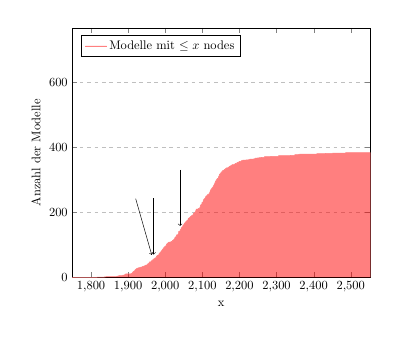
\begin{tikzpicture}[scale=0.45]
				\begin{axis}[
				xlabel = {x},
				ylabel = {Anzahl der Modelle},
				xmin = 1749,
				xmax = 2553,
				ymin = 0,
				ymax = 768,
				legend pos = north west,
				ymajorgrids = true,
				grid style = dashed,
				]
				\path[name path=axis] (axis cs:0,0) -- (axis cs:1,0);
				
				\addplot[color = red!50, fill=red, fill opacity=0.5]
				coordinates{
					(1749, 0)(1815.99, 0)(1816, 1)(1835.99, 1)(1836, 2)(1840.99, 2)(1841, 3)(1869.99, 3)(1870, 4)(1873.99, 4)(1874, 5)(1875.99, 5)(1876, 6)(1885.99, 6)(1886, 7)(1889.99, 7)(1890, 8)(1890.99, 8)(1891, 9)(1891.99, 9)(1892, 10)(1893.99, 10)(1894, 11)(1907.99, 11)(1908, 13)(1910.99, 13)(1911, 14)(1911.99, 14)(1912, 16)(1912.99, 16)(1913, 17)(1913.99, 17)(1914, 18)(1914.99, 18)(1915, 19)(1915.99, 19)(1916, 20)(1917.99, 20)(1918, 22)(1918.99, 22)(1919, 24)(1920.99, 24)(1921, 26)(1922.99, 26)(1923, 28)(1924.99, 28)(1925, 29)(1927.99, 29)(1928, 30)(1931.99, 30)(1932, 31)(1933.99, 31)(1934, 32)(1936.99, 32)(1937, 33)(1938.99, 33)(1939, 34)(1941.99, 34)(1942, 35)(1944.99, 35)(1945, 37)(1946.99, 37)(1947, 38)(1949.99, 38)(1950, 39)(1951.99, 39)(1952, 41)(1952.99, 41)(1953, 42)(1953.99, 42)(1954, 43)(1955.99, 43)(1956, 45)(1956.99, 45)(1957, 47)(1957.99, 47)(1958, 48)(1961.99, 48)(1962, 50)(1962.99, 50)(1963, 51)(1963.99, 51)(1964, 53)(1966.99, 53)(1967, 56)(1968.99, 56)(1969, 57)(1970.99, 57)(1971, 58)(1971.99, 58)(1972, 59)(1972.99, 59)(1973, 60)(1974.99, 60)(1975, 61)(1975.99, 61)(1976, 65)(1976.99, 65)(1977, 66)(1977.99, 66)(1978, 67)(1978.99, 67)(1979, 68)(1980.99, 68)(1981, 69)(1982.99, 69)(1983, 73)(1983.99, 73)(1984, 75)(1984.99, 75)(1985, 76)(1986.99, 76)(1987, 77)(1987.99, 77)(1988, 80)(1988.99, 80)(1989, 81)(1989.99, 81)(1990, 83)(1990.99, 83)(1991, 84)(1991.99, 84)(1992, 86)(1992.99, 86)(1993, 87)(1993.99, 87)(1994, 89)(1994.99, 89)(1995, 91)(1996.99, 91)(1997, 93)(1997.99, 93)(1998, 94)(1998.99, 94)(1999, 95)(1999.99, 95)(2000, 96)(2000.99, 96)(2001, 97)(2001.99, 97)(2002, 98)(2002.99, 98)(2003, 101)(2003.99, 101)(2004, 103)(2004.99, 103)(2005, 105)(2006.99, 105)(2007, 106)(2007.99, 106)(2008, 108)(2009.99, 108)(2010, 109)(2014.99, 109)(2015, 110)(2016.99, 110)(2017, 111)(2018.99, 111)(2019, 114)(2020.99, 114)(2021, 115)(2021.99, 115)(2022, 116)(2022.99, 116)(2023, 117)(2023.99, 117)(2024, 118)(2024.99, 118)(2025, 121)(2025.99, 121)(2026, 123)(2026.99, 123)(2027, 124)(2027.99, 124)(2028, 125)(2028.99, 125)(2029, 126)(2029.99, 126)(2030, 130)(2030.99, 130)(2031, 131)(2033.99, 131)(2034, 133)(2034.99, 133)(2035, 134)(2035.99, 134)(2036, 141)(2036.99, 141)(2037, 142)(2038.99, 142)(2039, 143)(2039.99, 143)(2040, 145)(2040.99, 145)(2041, 147)(2041.99, 147)(2042, 148)(2042.99, 148)(2043, 152)(2043.99, 152)(2044, 154)(2044.99, 154)(2045, 155)(2046.99, 155)(2047, 159)(2047.99, 159)(2048, 161)(2048.99, 161)(2049, 162)(2049.99, 162)(2050, 163)(2050.99, 163)(2051, 166)(2051.99, 166)(2052, 168)(2053.99, 168)(2054, 170)(2054.99, 170)(2055, 171)(2055.99, 171)(2056, 173)(2056.99, 173)(2057, 174)(2058.99, 174)(2059, 175)(2059.99, 175)(2060, 176)(2060.99, 176)(2061, 178)(2061.99, 178)(2062, 181)(2062.99, 181)(2063, 183)(2064.99, 183)(2065, 184)(2066.99, 184)(2067, 186)(2067.99, 186)(2068, 187)(2068.99, 187)(2069, 188)(2069.99, 188)(2070, 189)(2070.99, 189)(2071, 190)(2071.99, 190)(2072, 191)(2072.99, 191)(2073, 192)(2074.99, 192)(2075, 194)(2075.99, 194)(2076, 197)(2077.99, 197)(2078, 198)(2078.99, 198)(2079, 200)(2079.99, 200)(2080, 201)(2080.99, 201)(2081, 202)(2081.99, 202)(2082, 206)(2082.99, 206)(2083, 210)(2087.99, 210)(2088, 211)(2088.99, 211)(2089, 213)(2092.99, 213)(2093, 215)(2093.99, 215)(2094, 218)(2094.99, 218)(2095, 223)(2096.99, 223)(2097, 225)(2098.99, 225)(2099, 230)(2099.99, 230)(2100, 231)(2100.99, 231)(2101, 232)(2101.99, 232)(2102, 236)(2102.99, 236)(2103, 239)(2103.99, 239)(2104, 240)(2104.99, 240)(2105, 242)(2105.99, 242)(2106, 243)(2106.99, 243)(2107, 244)(2107.99, 244)(2108, 247)(2108.99, 247)(2109, 249)(2109.99, 249)(2110, 251)(2111.99, 251)(2112, 252)(2113.99, 252)(2114, 256)(2116.99, 256)(2117, 257)(2118.99, 257)(2119, 260)(2119.99, 260)(2120, 263)(2120.99, 263)(2121, 266)(2121.99, 266)(2122, 269)(2122.99, 269)(2123, 270)(2123.99, 270)(2124, 271)(2124.99, 271)(2125, 275)(2126.99, 275)(2127, 276)(2127.99, 276)(2128, 278)(2128.99, 278)(2129, 280)(2129.99, 280)(2130, 283)(2131.99, 283)(2132, 287)(2132.99, 287)(2133, 289)(2133.99, 289)(2134, 292)(2134.99, 292)(2135, 295)(2135.99, 295)(2136, 297)(2136.99, 297)(2137, 298)(2137.99, 298)(2138, 301)(2139.99, 301)(2140, 304)(2140.99, 304)(2141, 305)(2142.99, 305)(2143, 308)(2143.99, 308)(2144, 312)(2144.99, 312)(2145, 313)(2145.99, 313)(2146, 317)(2146.99, 317)(2147, 318)(2147.99, 318)(2148, 320)(2148.99, 320)(2149, 321)(2149.99, 321)(2150, 323)(2150.99, 323)(2151, 324)(2151.99, 324)(2152, 325)(2152.99, 325)(2153, 326)(2153.99, 326)(2154, 328)(2154.99, 328)(2155, 329)(2156.99, 329)(2157, 330)(2158.99, 330)(2159, 332)(2159.99, 332)(2160, 333)(2161.99, 333)(2162, 335)(2163.99, 335)(2164, 336)(2164.99, 336)(2165, 337)(2168.99, 337)(2169, 338)(2169.99, 338)(2170, 339)(2170.99, 339)(2171, 340)(2171.99, 340)(2172, 341)(2172.99, 341)(2173, 342)(2173.99, 342)(2174, 343)(2176.99, 343)(2177, 345)(2178.99, 345)(2179, 346)(2179.99, 346)(2180, 347)(2186.99, 347)(2187, 349)(2187.99, 349)(2188, 350)(2188.99, 350)(2189, 351)(2192.99, 351)(2193, 353)(2193.99, 353)(2194, 354)(2197.99, 354)(2198, 356)(2199.99, 356)(2200, 357)(2203.99, 357)(2204, 358)(2204.99, 358)(2205, 360)(2208.99, 360)(2209, 361)(2217.99, 361)(2218, 362)(2224.99, 362)(2225, 363)(2227.99, 363)(2228, 364)(2237.99, 364)(2238, 365)(2240.99, 365)(2241, 366)(2242.99, 366)(2243, 367)(2248.99, 367)(2249, 368)(2253.99, 368)(2254, 369)(2258.99, 369)(2259, 370)(2266.99, 370)(2267, 371)(2267.99, 371)(2268, 372)(2284.99, 372)(2285, 373)(2304.99, 373)(2305, 374)(2305.99, 374)(2306, 375)(2336.99, 375)(2337, 376)(2348.99, 376)(2349, 377)(2349.99, 377)(2350, 378)(2359.99, 378)(2360, 379)(2361.99, 379)(2362, 380)(2408.99, 380)(2409, 381)(2431.99, 381)(2432, 382)(2450.99, 382)(2451, 383)(2485.99, 383)(2486, 384)(2553, 384)(2553, 0)
				};
				
				\node[rotate = 90](source) at(axis cs:1917,256) { \mmfh };
				\node(destination) at(axis cs:1967,56) {};
				\draw[->](source)--(destination);
				
				\node[rotate = 90](source2) at(axis cs:2040,345) { \wph };
				\node(destination2) at(axis cs:2040,145) {};
				\draw[->](source2)--(destination2);
				
				\node[rotate = 90](source3) at(axis cs:1969,257) { \rnh };
				\node(destination3) at(axis cs:1969,57) {};
				\draw[->](source3)--(destination3);
				
				\addlegendentry{Modelle mit $\leq x$ nodes}
				
				\end{axis}
				\end{tikzpicture}
				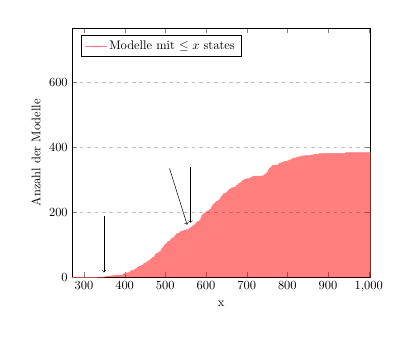
\begin{tikzpicture}[scale=0.45]
				\begin{axis}[
				xlabel = {x},
				ylabel = {Anzahl der Modelle},
				xmin = 270.9,
				xmax = 1004.1,
				ymin = 0,
				ymax = 768,
				legend pos = north west,
				ymajorgrids = true,
				grid style = dashed,
				]
				\path[name path=axis] (axis cs:0,0) -- (axis cs:1,0);
				
				\addplot[color = red!50, fill=red, fill opacity=0.5]
				coordinates{
					(270.9, 0)(331.99, 0)(332, 1)(348.99, 1)(349, 2)(352.99, 2)(353, 3)(357.99, 3)(358, 4)(365.99, 4)(366, 5)(370.99, 5)(371, 6)(376.99, 6)(377, 7)(393.99, 7)(394, 8)(395.99, 8)(396, 10)(397.99, 10)(398, 12)(401.99, 12)(402, 13)(403.99, 13)(404, 14)(408.99, 14)(409, 15)(410.99, 15)(411, 16)(412.99, 16)(413, 17)(414.99, 17)(415, 20)(416.99, 20)(417, 22)(422.99, 22)(423, 23)(423.99, 23)(424, 24)(424.99, 24)(425, 25)(426.99, 25)(427, 27)(429.99, 27)(430, 28)(430.99, 28)(431, 30)(431.99, 30)(432, 31)(432.99, 31)(433, 32)(433.99, 32)(434, 33)(435.99, 33)(436, 34)(436.99, 34)(437, 35)(439.99, 35)(440, 36)(441.99, 36)(442, 37)(442.99, 37)(443, 38)(443.99, 38)(444, 39)(445.99, 39)(446, 42)(447.99, 42)(448, 44)(451.99, 44)(452, 45)(452.99, 45)(453, 47)(454.99, 47)(455, 49)(456.99, 49)(457, 50)(458.99, 50)(459, 51)(460.99, 51)(461, 53)(461.99, 53)(462, 54)(462.99, 54)(463, 55)(464.99, 55)(465, 57)(465.99, 57)(466, 58)(466.99, 58)(467, 59)(467.99, 59)(468, 61)(469.99, 61)(470, 62)(472.99, 62)(473, 64)(473.99, 64)(474, 67)(474.99, 67)(475, 68)(475.99, 68)(476, 71)(476.99, 71)(477, 73)(477.99, 73)(478, 74)(478.99, 74)(479, 75)(482.99, 75)(483, 77)(484.99, 77)(485, 78)(485.99, 78)(486, 79)(486.99, 79)(487, 80)(488.99, 80)(489, 83)(489.99, 83)(490, 85)(490.99, 85)(491, 88)(491.99, 88)(492, 90)(492.99, 90)(493, 91)(493.99, 91)(494, 92)(494.99, 92)(495, 94)(495.99, 94)(496, 95)(496.99, 95)(497, 98)(497.99, 98)(498, 100)(498.99, 100)(499, 101)(499.99, 101)(500, 103)(502.99, 103)(503, 105)(503.99, 105)(504, 106)(504.99, 106)(505, 109)(505.99, 109)(506, 110)(507.99, 110)(508, 111)(509.99, 111)(510, 112)(511.99, 112)(512, 114)(512.99, 114)(513, 115)(513.99, 115)(514, 120)(516.99, 120)(517, 121)(518.99, 121)(519, 122)(519.99, 122)(520, 123)(521.99, 123)(522, 125)(522.99, 125)(523, 127)(523.99, 127)(524, 129)(525.99, 129)(526, 131)(526.99, 131)(527, 132)(527.99, 132)(528, 135)(531.99, 135)(532, 136)(533.99, 136)(534, 137)(535.99, 137)(536, 139)(536.99, 139)(537, 141)(538.99, 141)(539, 142)(539.99, 142)(540, 143)(544.99, 143)(545, 145)(546.99, 145)(547, 146)(550.99, 146)(551, 147)(556.99, 147)(557, 149)(558.99, 149)(559, 150)(559.99, 150)(560, 151)(560.99, 151)(561, 152)(561.99, 152)(562, 155)(564.99, 155)(565, 156)(565.99, 156)(566, 158)(566.99, 158)(567, 159)(569.99, 159)(570, 160)(570.99, 160)(571, 161)(571.99, 161)(572, 163)(572.99, 163)(573, 164)(573.99, 164)(574, 165)(574.99, 165)(575, 166)(575.99, 166)(576, 168)(576.99, 168)(577, 169)(577.99, 169)(578, 170)(578.99, 170)(579, 172)(579.99, 172)(580, 173)(583.99, 173)(584, 175)(585.99, 175)(586, 180)(587.99, 180)(588, 185)(588.99, 185)(589, 186)(589.99, 186)(590, 192)(590.99, 192)(591, 193)(592.99, 193)(593, 195)(593.99, 195)(594, 196)(594.99, 196)(595, 197)(596.99, 197)(597, 198)(597.99, 198)(598, 200)(598.99, 200)(599, 202)(600.99, 202)(601, 203)(603.99, 203)(604, 205)(606.99, 205)(607, 207)(607.99, 207)(608, 209)(610.99, 209)(611, 210)(611.99, 210)(612, 212)(612.99, 212)(613, 214)(613.99, 214)(614, 217)(614.99, 217)(615, 219)(615.99, 219)(616, 221)(616.99, 221)(617, 224)(617.99, 224)(618, 225)(618.99, 225)(619, 226)(619.99, 226)(620, 227)(620.99, 227)(621, 228)(621.99, 228)(622, 229)(622.99, 229)(623, 231)(623.99, 231)(624, 232)(624.99, 232)(625, 234)(627.99, 234)(628, 235)(629.99, 235)(630, 236)(630.99, 236)(631, 237)(631.99, 237)(632, 238)(632.99, 238)(633, 239)(633.99, 239)(634, 240)(634.99, 240)(635, 243)(635.99, 243)(636, 246)(637.99, 246)(638, 248)(638.99, 248)(639, 250)(639.99, 250)(640, 252)(640.99, 252)(641, 253)(641.99, 253)(642, 255)(642.99, 255)(643, 258)(647.99, 258)(648, 259)(648.99, 259)(649, 260)(650.99, 260)(651, 262)(651.99, 262)(652, 263)(652.99, 263)(653, 265)(653.99, 265)(654, 266)(654.99, 266)(655, 269)(656.99, 269)(657, 271)(657.99, 271)(658, 272)(660.99, 272)(661, 273)(661.99, 273)(662, 276)(666.99, 276)(667, 277)(670.99, 277)(671, 278)(672.99, 278)(673, 279)(673.99, 279)(674, 283)(675.99, 283)(676, 285)(679.99, 285)(680, 289)(680.99, 289)(681, 290)(683.99, 290)(684, 292)(686.99, 292)(687, 294)(687.99, 294)(688, 295)(689.99, 295)(690, 299)(692.99, 299)(693, 301)(695.99, 301)(696, 303)(699.99, 303)(700, 304)(708.99, 304)(709, 307)(711.99, 307)(712, 309)(712.99, 309)(713, 310)(714.99, 310)(715, 311)(716.99, 311)(717, 312)(735.99, 312)(736, 313)(741.99, 313)(742, 315)(743.99, 315)(744, 317)(744.99, 317)(745, 318)(746.99, 318)(747, 319)(748.99, 319)(749, 323)(751.99, 323)(752, 327)(752.99, 327)(753, 331)(754.99, 331)(755, 332)(755.99, 332)(756, 336)(756.99, 336)(757, 337)(759.99, 337)(760, 340)(760.99, 340)(761, 341)(761.99, 341)(762, 343)(762.99, 343)(763, 344)(763.99, 344)(764, 345)(765.99, 345)(766, 346)(777.99, 346)(778, 348)(778.99, 348)(779, 349)(779.99, 349)(780, 351)(781.99, 351)(782, 352)(783.99, 352)(784, 353)(786.99, 353)(787, 354)(790.99, 354)(791, 356)(791.99, 356)(792, 357)(797.99, 357)(798, 358)(799.99, 358)(800, 359)(802.99, 359)(803, 360)(803.99, 360)(804, 361)(805.99, 361)(806, 362)(808.99, 362)(809, 363)(809.99, 363)(810, 365)(812.99, 365)(813, 366)(813.99, 366)(814, 367)(821.99, 367)(822, 369)(824.99, 369)(825, 370)(825.99, 370)(826, 371)(830.99, 371)(831, 372)(831.99, 372)(832, 373)(836.99, 373)(837, 374)(843.99, 374)(844, 375)(855.99, 375)(856, 376)(858.99, 376)(859, 377)(864.99, 377)(865, 378)(866.99, 378)(867, 379)(876.99, 379)(877, 380)(877.99, 380)(878, 381)(898.99, 381)(899, 382)(940.99, 382)(941, 383)(942.99, 383)(943, 384)(1004.1, 384)(1004.1, 0)
				};
				
				\node[rotate = 90](source) at(axis cs:349,202) { \mmfh };
				\node(destination) at(axis cs:349,2) {};
				\draw[->](source)--(destination);
				
				\node[rotate = 90](source2) at(axis cs:562,355) { \wph };
				\node(destination2) at(axis cs:562,155) {};
				\draw[->](source2)--(destination2);
				
				\node[rotate = 90](source3) at(axis cs:507,349) { \rnh };
				\node(destination3) at(axis cs:557,149) {};
				\draw[->](source3)--(destination3);
				
				\addlegendentry{Modelle mit $\leq x$ states}
				
				\end{axis}
				\end{tikzpicture}
			}
		}
	\end{center}
	\begin{center}
		\makebox[0pt]{
			\begin{tabular}{|l|cc|cc|r|}
				\hline
				\textbf{} & \textbf{\#nodes} & \textbf{\% reduction} & \textbf{\#states} & \textbf{\% reduction} & \textbf{Zeit} \\
				\hline
				originales Modell & 2714 & { \color{gray} 0\%} & 3045 & { \color{gray} 0\%} & 12s \\
				\hline
				Maximum Merge First & 1967 & 28\% & 349 & 89\% & 7s \\
				Remove Nodes & 1969 & 27\% & 557 & 82\% & 6s \\
				Welsh-Powell & 2040 & 25\% & 562 & 82\% & 6s \\
				max. Reduktion & 1816 & 33\% & 332 & 89\% & \\
				\hline
			\end{tabular}
		}
	\end{center}
\end{figure}


\begin{comment}

\begin{figure}
	\caption{Verteilung der nodes und states von Modell 8}
	%\label{}
	\begin{center}
	\scalebox{2}{
	\hspace{-14ex}	
	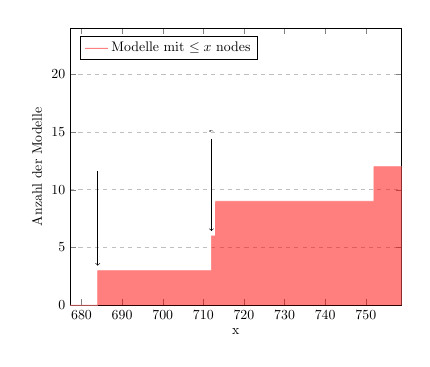
\begin{tikzpicture}[scale=0.5]
	\begin{axis}[
	xlabel = {x},
	ylabel = {Anzahl der Modelle},
	xmin = 677.2,
	xmax = 758.8,
	ymin = 0,
	ymax = 24,
	legend pos = north west,
	ymajorgrids = true,
	grid style = dashed,
	]
	\path[name path=axis] (axis cs:0,0) -- (axis cs:1,0);
	
	\addplot[color = red!50, fill=red, fill opacity=0.5]
	coordinates{
		(677.2, 0)(683.99, 0)(684, 3)(711.99, 3)(712, 6)(712.99, 6)(713, 9)(751.99, 9)(752, 12)(758.8, 12)(758.8, 0)
	};

	\node[rotate=90] (source) at (axis cs:712,15){\mmfh, \wph};
	\node (destination) at (axis cs:712,6){};
	\draw[->](source)--(destination);
	
	\node[rotate=90] (source2) at (axis cs:684,12){\rnh};
	\node (destination2) at (axis cs:684,3){};
	\draw[->](source2)--(destination2);	
	
	
	\addlegendentry{Modelle mit $\leq x$ nodes}
	
	\end{axis}
	\end{tikzpicture}
	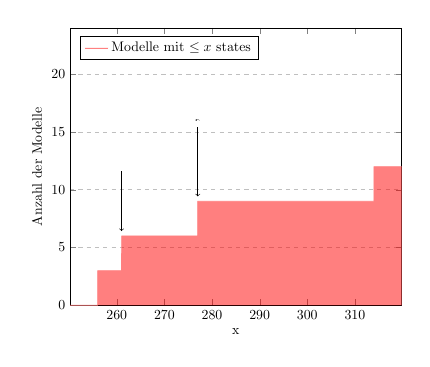
\begin{tikzpicture}[scale=0.5]
	\begin{axis}[
	xlabel = {x},
	ylabel = {Anzahl der Modelle},
	xmin = 250.2,
	xmax = 319.8,
	ymin = 0,
	ymax = 24,
	legend pos = north west,
	ymajorgrids = true,
	grid style = dashed,
	]
	\path[name path=axis] (axis cs:0,0) -- (axis cs:1,0);
	
	\addplot[color = red!50, fill=red, fill opacity=0.5]
	coordinates{
		(250.2, 0)(255.99, 0)(256, 3)(260.99, 3)(261, 6)(276.99, 6)(277, 9)(313.99, 9)(314, 12)(319.8, 12)(319.8, 0)
	};
	
	\node[rotate=90] (source) at (axis cs:277,16){\mmfh, \wph};
	\node (destination) at (axis cs:277,9){};
	\draw[->](source)--(destination);
	
	\node[rotate=90] (source2) at (axis cs:261,12){\rnh};
	\node (destination2) at (axis cs:261,6){};
	\draw[->](source2)--(destination2);	
	
	
	\addlegendentry{Modelle mit $\leq x$ states}
	
	\end{axis}
	\end{tikzpicture}
}
\end{center}

\begin{center}
	\begin{tabular}{|l|ccr|}
		\hline
		\textbf{} & \textbf{\#nodes} & \textbf{\#states} & \textbf{Zeit} \\
		\hline
		originales Modell & 866  & 123 & 7s \\
		\hline
		Maximum Merge First & 712 & 277 & 6s \\
		Remove Nodes & 684 & 261 & 4s \\
		Welsh-Powell & 712 & 277 & 3s \\
		Minimum (red. Modelle) & 684 & 256 &  \\
		\hline
	\end{tabular}
\end{center}
\end{figure}



	
\begin{figure}
	\caption{Verteilung der nodes und states von Modell 10}
	%\label{}
	\begin{center}
	\scalebox{2}{
	\hspace{-14ex}	
	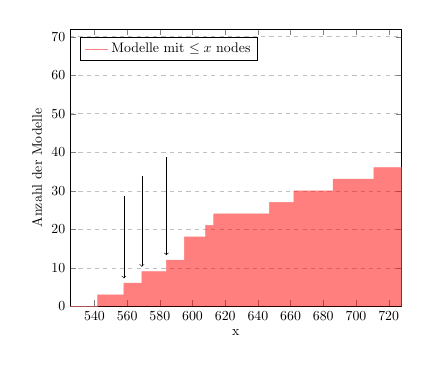
\begin{tikzpicture}[scale=0.5]
	\begin{axis}[
	xlabel = {x},
	ylabel = {Anzahl der Modelle},
	xmin = 525.1,
	xmax = 727.9,
	ymin = 0,
	ymax = 72,
	legend pos = north west,
	ymajorgrids = true,
	grid style = dashed,
	]
	\path[name path=axis] (axis cs:0,0) -- (axis cs:1,0);
	
	\addplot[color = red!50, fill=red, fill opacity=0.5]
	coordinates{
		(525.1, 0)(541.99, 0)(542, 3)(557.99, 3)(558, 6)(568.99, 6)(569, 9)(583.99, 9)(584, 12)(594.99, 12)(595, 18)(607.99, 18)(608, 21)(612.99, 21)(613, 24)(646.99, 24)(647, 27)(661.99, 27)(662, 30)(685.99, 30)(686, 33)(710.99, 33)(711, 36)(727.9, 36)(727.9, 0)
	};
	
	\node[rotate=90] (source) at (axis cs:558,30){\mmfh};
	\node (destination) at (axis cs:558,6){};
	\draw[->](source)--(destination);
	
	\node[rotate=90] (source2) at (axis cs:569,35){\wph};
	\node (destination2) at (axis cs:569,9){};
	\draw[->](source2)--(destination2);	
	
	\node[rotate=90] (source3) at (axis cs:584,40){\rnh};
	\node (destination3) at (axis cs:584,12){};
	\draw[->](source3)--(destination3);
	
	\addlegendentry{Modelle mit $\leq x$ nodes}
	
	\end{axis}
	\end{tikzpicture}
	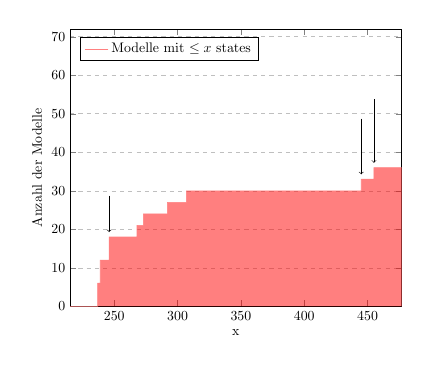
\begin{tikzpicture}[scale=0.5]
	\begin{axis}[
	xlabel = {x},
	ylabel = {Anzahl der Modelle},
	xmin = 215.2,
	xmax = 476.8,
	ymin = 0,
	ymax = 72,
	legend pos = north west,
	ymajorgrids = true,
	grid style = dashed,
	]
	\path[name path=axis] (axis cs:0,0) -- (axis cs:1,0);
	
	\addplot[color = red!50, fill=red, fill opacity=0.5]
	coordinates{
		(215.2, 0)(236.99, 0)(237, 6)(238.99, 6)(239, 12)(245.99, 12)(246, 18)(267.99, 18)(268, 21)(272.99, 21)(273, 24)(291.99, 24)(292, 27)(306.99, 27)(307, 30)(444.99, 30)(445, 33)(454.99, 33)(455, 36)(476.8, 36)(476.8, 0)
	};

	\node[rotate=90] (source) at (axis cs:445,50){\mmfh};
	\node (destination) at (axis cs:445,33){};
	\draw[->](source)--(destination);
	
	\node[rotate=90] (source2) at (axis cs:455,55){\wph};
	\node (destination2) at (axis cs:455,36){};
	\draw[->](source2)--(destination2);	
	
	\node[rotate=90] (source3) at (axis cs:246,30){\rnh};
	\node (destination3) at (axis cs:246,18){};
	\draw[->](source3)--(destination3);
	
	\addlegendentry{Modelle mit $\leq x$ states}
	
	\end{axis}
	\end{tikzpicture}
}
\end{center}

\begin{center}
	\begin{tabular}{|l|ccr|}
		\hline
		\textbf{} & \textbf{\#nodes} & \textbf{\#states} & \textbf{Zeit} \\
		\hline
		originales Modell & 714 & 113  & 3s \\
		\hline
		Maximum Merge First & 558 & 445 & 4s  \\
		Remove Nodes & 584 & 246 &  6s \\
		Welsh-Powell & 569 & 455 & 4s \\
		Minimum (red. Modelle) & 542 & 237 &  \\
		\hline
	\end{tabular}
\end{center}

\end{figure}
\end{comment}



\begin{figure}
	\caption{Verteilung der nodes und states von Modell 11}
	\label{model11}
	\begin{center}
		\scalebox{2}{
			\makebox[0pt]{
				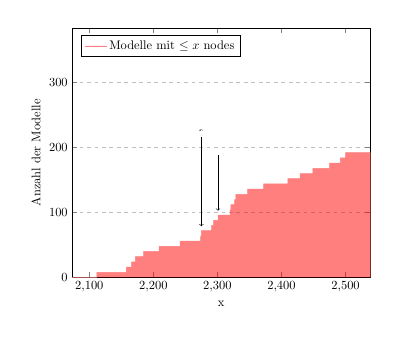
\begin{tikzpicture}[scale=0.45]
				\begin{axis}[
				xlabel = {x},
				ylabel = {Anzahl der Modelle},
				xmin = 2073.2,
				xmax = 2538.8,
				ymin = 0,
				ymax = 384,
				legend pos = north west,
				ymajorgrids = true,
				grid style = dashed,
				]
				\path[name path=axis] (axis cs:0,0) -- (axis cs:1,0);
				
				\addplot[color = red!50, fill=red, fill opacity=0.5]
				coordinates{
					(2073.2, 0)(2111.99, 0)(2112, 8)(2157.99, 8)(2158, 16)(2165.99, 16)(2166, 24)(2171.99, 24)(2172, 32)(2184.99, 32)(2185, 40)(2208.99, 40)(2209, 48)(2241.99, 48)(2242, 56)(2273.99, 56)(2274, 64)(2274.99, 64)(2275, 72)(2290.99, 72)(2291, 80)(2293.99, 80)(2294, 88)(2300.99, 88)(2301, 96)(2319.99, 96)(2320, 104)(2320.99, 104)(2321, 112)(2326.99, 112)(2327, 120)(2328.99, 120)(2329, 128)(2346.99, 128)(2347, 136)(2371.99, 136)(2372, 144)(2409.99, 144)(2410, 152)(2428.99, 152)(2429, 160)(2448.99, 160)(2449, 168)(2474.99, 168)(2475, 176)(2491.99, 176)(2492, 184)(2499.99, 184)(2500, 192)(2538.8, 192)(2538.8, 0)
				};
				
				\node[rotate = 90](source) at(axis cs:2275,225) { \mmfh, \wph };
				\node(destination) at(axis cs:2275,72) {};
				\draw[->](source)--(destination);
				
				\node[rotate = 90](source3) at(axis cs:2301,196) { \rnh };
				\node(destination3) at(axis cs:2301,96) {};
				\draw[->](source3)--(destination3);
				
				\addlegendentry{Modelle mit $\leq x$ nodes}
				
				\end{axis}
				\end{tikzpicture}
				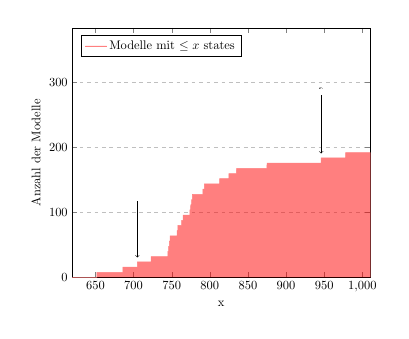
\begin{tikzpicture}[scale=0.45]
				\begin{axis}[
				xlabel = {x},
				ylabel = {Anzahl der Modelle},
				xmin = 619.4,
				xmax = 1010.6,
				ymin = 0,
				ymax = 384,
				legend pos = north west,
				ymajorgrids = true,
				grid style = dashed,
				]
				\path[name path=axis] (axis cs:0,0) -- (axis cs:1,0);
				
				\addplot[color = red!50, fill=red, fill opacity=0.5]
				coordinates{
					(619.4, 0)(651.99, 0)(652, 8)(685.99, 8)(686, 16)(704.99, 16)(705, 24)(722.99, 24)(723, 32)(744.99, 32)(745, 40)(745.99, 40)(746, 48)(746.99, 48)(747, 56)(747.99, 56)(748, 64)(756.99, 64)(757, 72)(757.99, 72)(758, 80)(762.99, 80)(763, 88)(764.99, 88)(765, 96)(773.99, 96)(774, 104)(774.99, 104)(775, 112)(775.99, 112)(776, 120)(776.99, 120)(777, 128)(790.99, 128)(791, 136)(792.99, 136)(793, 144)(812.99, 144)(813, 152)(824.99, 152)(825, 160)(834.99, 160)(835, 168)(874.99, 168)(875, 176)(945.99, 176)(946, 184)(977.99, 184)(978, 192)(1010.6, 192)(1010.6, 0)
				};
				
				\node[rotate = 90](source) at(axis cs:946,290) { \mmfh, \wph };
				\node(destination) at(axis cs:946,184) {};
				\draw[->](source)--(destination);

				\node[rotate = 90](source3) at(axis cs:705,124) { \rnh };
				\node(destination3) at(axis cs:705,24) {};
				\draw[->](source3)--(destination3);
				
				\addlegendentry{Modelle mit $\leq x$ states}
				
				\end{axis}
				\end{tikzpicture}
			}
		}
	\end{center}
	\begin{center}
		\makebox[0pt]{
			\begin{tabular}{|l|cc|cc|r|}
				\hline
				\textbf{} & \textbf{\#nodes} & \textbf{\% reduction} & \textbf{\#states} & \textbf{\% reduction} & \textbf{Zeit} \\
				\hline
				originales Modell & 2285 & { \color{gray} 0\%} & 3440 & { \color{gray} 0\%} & 8s \\
				\hline
				Maximum Merge First & 2275 & 0.4\% & 946 & 73\% & 8s \\
				Remove Nodes & 2301 & -1\% & 705 & 80\% & 9s \\
				Welsh-Powell & 2275 & 0.4\% & 946 & 73\% & 8s \\
				max. Reduktion & 2112 & 8\% & 652 & 81\% & \\
				\hline
			\end{tabular}
		}
	\end{center}
\end{figure}


\begin{comment}
	
\begin{figure}
	\caption{Verteilung der nodes und states von Modell 12}
	\begin{center}
	\scalebox{2}{
		\hspace{-14ex}	
	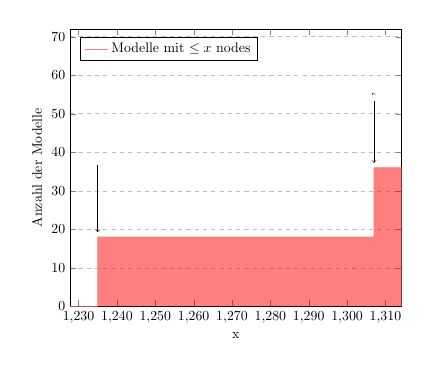
\begin{tikzpicture}[scale=0.5]
	\begin{axis}[
	xlabel = {x},
	ylabel = {Anzahl der Modelle},
	xmin = 1227.8,
	xmax = 1314.2,
	ymin = 0,
	ymax = 72,
	legend pos = north west,
	ymajorgrids = true,
	grid style = dashed,
	]
	\path[name path=axis] (axis cs:0,0) -- (axis cs:1,0);
	
	\addplot[color = red!50, fill=red, fill opacity=0.5]
	coordinates{
		(1227.8, 0)(1234.99, 0)(1235, 18)(1306.99, 18)(1307, 36)(1314.2, 36)(1314.2, 0)
	};
	
	\node[rotate=90] (source) at (axis cs:1235,38){\mmfh};
	\node (destination) at (axis cs:1235,18){};
	\draw[->](source)--(destination);
	
	\node[rotate=90] (source2) at (axis cs:1307,55){\wph, \rnh};
	\node (destination2) at (axis cs:1307,36){};
	\draw[->](source2)--(destination2);	
	
	\addlegendentry{Modelle mit $\leq x$ nodes};
	
	\end{axis}
	\end{tikzpicture}
	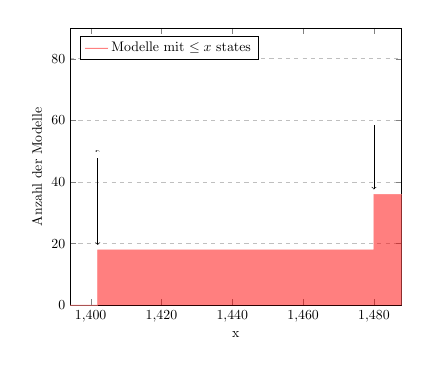
\begin{tikzpicture}[scale=0.5]
	\begin{axis}[
	xlabel = {x},
	ylabel = {Anzahl der Modelle},
	xmin = 1394.2,
	xmax = 1487.8,
	ymin = 0,
	ymax = 90,
	legend pos = north west,
	ymajorgrids = true,
	grid style = dashed,
	]
	\path[name path=axis] (axis cs:0,0) -- (axis cs:1,0);
	
	\addplot[color = red!50, fill=red, fill opacity=0.5]
	coordinates{
		(1394.2, 0)(1401.99, 0)(1402, 18)(1479.99, 18)(1480, 36)(1487.8, 36)(1487.8, 0)
	};
	
	\node[rotate=90] (source) at (axis cs:1480,60){\mmfh};
	\node (destination) at (axis cs:1480,36){};
	\draw[->](source)--(destination);

	\node[rotate=90] (source2) at (axis cs:1402,50){\wph, \rnh};
	\node (destination2) at (axis cs:1402,18){};
	\draw[->](source2)--(destination2);	

	\addlegendentry{Modelle mit $\leq x$ states}
	
	\end{axis}
	\end{tikzpicture}
}
\end{center}
\begin{center}
	\begin{tabular}{|l|ccr|}
		\hline
		\textbf{} & \textbf{\#nodes} & \textbf{\#states} & \textbf{Zeit} \\
		\hline
		originales Modell & 1278 & 257 & 15s \\
		\hline
		Maximum Merge First & 1235 & 1480 & 3s  \\
		Remove Nodes & 1307 & 1402 &  5s \\
		Welsh-Powell & 1307 & 1402 & 6s \\
		Minimum (red. Modelle) & 1235 & 1402 &  \\
		\hline
	\end{tabular}
\end{center}
\end{figure}
\end{comment}


\begin{figure}
	\caption{Verteilung der nodes und states von Modell 18}
	\label{model18}
	\begin{center}
		\scalebox{2}{
			\makebox[0pt]{
				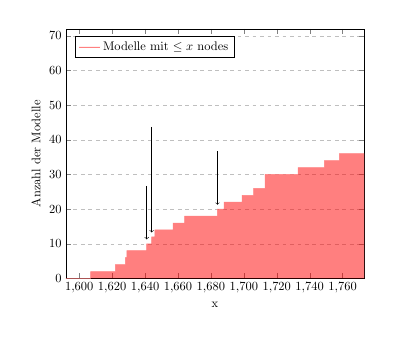
\begin{tikzpicture}[scale=0.45]
				\begin{axis}[
				xlabel = {x},
				ylabel = {Anzahl der Modelle},
				xmin = 1591.9,
				xmax = 1773.1,
				ymin = 0,
				ymax = 72,
				legend pos = north west,
				ymajorgrids = true,
				grid style = dashed,
				]
				\path[name path=axis] (axis cs:0,0) -- (axis cs:1,0);
				
				\addplot[color = red!50, fill=red, fill opacity=0.5]
				coordinates{
					(1591.9, 0)(1606.99, 0)(1607, 2)(1621.99, 2)(1622, 4)(1627.99, 4)(1628, 6)(1628.99, 6)(1629, 8)(1640.99, 8)(1641, 10)(1643.99, 10)(1644, 12)(1645.99, 12)(1646, 14)(1656.99, 14)(1657, 16)(1663.99, 16)(1664, 18)(1683.99, 18)(1684, 20)(1687.99, 20)(1688, 22)(1698.99, 22)(1699, 24)(1705.99, 24)(1706, 26)(1712.99, 26)(1713, 30)(1732.99, 30)(1733, 32)(1748.99, 32)(1749, 34)(1757.99, 34)(1758, 36)(1773.1, 36)(1773.1, 0)
				};
				
				\node[rotate = 90](source) at(axis cs:1644,45) { \mmfh };
				\node(destination) at(axis cs:1644,12) {};
				\draw[->](source)--(destination);
				
				\node[rotate = 90](source2) at(axis cs:1641,28) { \wph };
				\node(destination2) at(axis cs:1641,10) {};
				\draw[->](source2)--(destination2);
				
				\node[rotate = 90](source3) at(axis cs:1684,38) { \rnh };
				\node(destination3) at(axis cs:1684,20) {};
				\draw[->](source3)--(destination3);
				
				\addlegendentry{Modelle mit $\leq x$ nodes}
				
				\end{axis}
				\end{tikzpicture}
				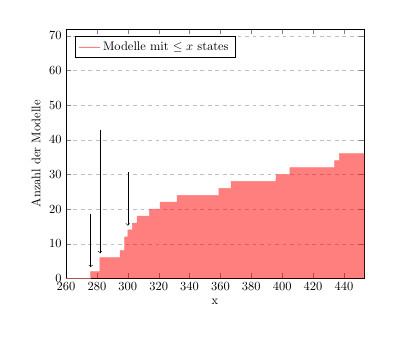
\begin{tikzpicture}[scale=0.45]
				\begin{axis}[
				xlabel = {x},
				ylabel = {Anzahl der Modelle},
				xmin = 259.9,
				xmax = 453.1,
				ymin = 0,
				ymax = 72,
				legend pos = north west,
				ymajorgrids = true,
				grid style = dashed,
				]
				\path[name path=axis] (axis cs:0,0) -- (axis cs:1,0);
				
				\addplot[color = red!50, fill=red, fill opacity=0.5]
				coordinates{
					(259.9, 0)(275.99, 0)(276, 2)(281.99, 2)(282, 6)(294.99, 6)(295, 8)(297.99, 8)(298, 12)(299.99, 12)(300, 14)(302.99, 14)(303, 16)(305.99, 16)(306, 18)(313.99, 18)(314, 20)(320.99, 20)(321, 22)(331.99, 22)(332, 24)(358.99, 24)(359, 26)(366.99, 26)(367, 28)(395.99, 28)(396, 30)(404.99, 30)(405, 32)(433.99, 32)(434, 34)(436.99, 34)(437, 36)(453.1, 36)(453.1, 0)
				};
				
				\node[rotate = 90](source) at(axis cs:300,32) { \mmfh };
				\node(destination) at(axis cs:300,14) {};
				\draw[->](source)--(destination);
				
				\node[rotate = 90](source2) at(axis cs:282,44) { \wph };
				\node(destination2) at(axis cs:282,6) {};
				\draw[->](source2)--(destination2);
				
				\node[rotate = 90](source3) at(axis cs:276,20) { \rnh };
				\node(destination3) at(axis cs:276,2) {};
				\draw[->](source3)--(destination3);
				
				\addlegendentry{Modelle mit $\leq x$ states}
				
				\end{axis}
				\end{tikzpicture}
			}
		}
	\end{center}
	\begin{center}
		\makebox[0pt]{
			\begin{tabular}{|l|cc|cc|r|}
				\hline
				\textbf{} & \textbf{\#nodes} & \textbf{\% reduction} & \textbf{\#states} & \textbf{\% reduction} & \textbf{Zeit} \\
				\hline
				originales Modell & 2215 & { \color{gray} 0\%} & 1010 & { \color{gray} 0\%} & 5s \\
				\hline
				Maximum Merge First & 1644 & 26\% & 300 & 70\% & 3s \\
				Remove Nodes & 1684 & 24\% & 276 & 73\% & 2s \\
				Welsh-Powell & 1641 & 26\% & 282 & 72\% & 3s \\
				max. Reduktion & 1607 & 27\% & 276 & 73\% & \\
				\hline
			\end{tabular}
		}
	\end{center}
\end{figure}

\begin{figure}
	\caption{Tabelle für Modell \texttt{in\_family.prism}}
	\label{familymodel}
	\label{last-diagram}
	\begin{center}
		\makebox[0pt]{
			\begin{tabular}{|l|cc|cc|r|}
				\hline
				\textbf{} & \textbf{\#nodes} & \textbf{\% reduction} & \textbf{\#states} & \textbf{\% reduction} & \textbf{Zeit} \\
				\hline
				originales Modell & 52057 & { \color{gray} 0\%} & 154201068 & { \color{gray} 0\%} & 122min \\
				\hline
				Remove Nodes & 37698 & 28\% & 13882176 & 91\% & 53min \\
				Welsh-Powell & 32757 & 37\% & 11609100 & 92\% & 48min \\
				\hline
			\end{tabular}
		}
	\end{center}
\end{figure}


\subsection{Offene Fragestellungen}

Wir wollen einmal kurz auf eine offene Fragestellung eingehen, die näher untersucht werden könnte:
Die vorgestellen Heuristiken zum Finden einer Graph\-färbung führen nicht zu einem eindeutigen Ergebnis.
Vielmehr erlauben sie nichtdeterministische Entscheidungen zum Beispiel beim Auswählen eines Knotens mit kleinster Nachbarschaft bei Variante \textins{Remove Nodes}.
Daher wäre es interessant zu einer Heuristik einmal alle möglichen entstehenden Modelle aufzulisten, die bei verschiedener Auflösung des enthaltenenen Nichtdeterminismus entstehen können.
Ein Extremfall, welcher dabei auftreten könnte, wäre, dass eine Heuristik allein bereits Modelle erzeugt, die sich über das gesamte Intervall der Anzahl von nodes bzw. states erstreckt.
Eine solche Heuristik wäre nutzlos, um innerhalb aller Modelle mit minimaler Zahl an Variablen ein optimales zu finden, wohl aber eventuell nützlich, um überhaupt ein Modell mit minimaler Zahl an Variablen zu finden.
Des Weiteren stellt sich die Frage, unter welchen Bedingungen die vorgestellten Heuristiken zu einem reduzierten Modell führen, welches mehr Variablen verwendet als erforderlich und wie ggf. solche Fälle in Software geschickt erkannt werden können.


\printbibliography

\end{document}